% Questo file definisce lo stile che verrà applicato
% ad ogni pagina di contenuto
\documentclass[a4paper,11pt]{article}

\usepackage{ifthen}
\usepackage[
 a4paper,
 top=2.5cm,
 bottom=2.5cm,
 left=1.5cm,
 right=1.5cm,
 head=30pt
]{geometry}
\usepackage[italian]{babel}
\usepackage[utf8x]{inputenc}
\usepackage[T1]{fontenc}
\usepackage{fancyhdr}
\usepackage[colorlinks=true, urlcolor=black, citecolor=black, linkcolor=black]{hyperref}
\usepackage{tabularx}
\usepackage{multirow}
\usepackage{booktabs}
\usepackage{color}
\usepackage[dvipsnames]{xcolor}
\usepackage{graphicx}
\usepackage{eurosym}
\usepackage{amsmath}
\usepackage{relsize}
\usepackage{placeins}
\usepackage{ltablex}
\usepackage{float}

\usepackage[multidot]{grffile}
\usepackage{xcolor,colortbl}
\definecolor{lightblue}{HTML}{56B4E6}
\definecolor{blue}{HTML}{2953A1}
\definecolor{darkblue}{HTML}{1E396E}
\usepackage{longtable}

\usepackage[toc,page]{appendix}
\renewcommand\appendixtocname{Appendice}
\renewcommand{\appendixpagename}{Appendice}

\newcommand\pagenumberingnoreset[1]{\gdef\thepage{\csname @#1\endcsname\c@page}}

% Cambia il font 
\renewcommand*\rmdefault{qhv}

% ***STILE PAGINA***
\pagestyle{fancy}
\fancyhf{}
\setlength{\headheight}{1cm} 
% No indentazione paragrafo
\setlength{\parindent}{0pt}

% ***INTESTAZIONE***
\newcommand\textline[4][t]{%
  \noindent\parbox[#1]{.333\textwidth}{\raisebox{-0.40\height}{#2}}%
  \parbox[#1]{.333\textwidth}{\centering #3}%
  \parbox[#1]{.333\textwidth}{\raggedleft #4}%
}

\lhead{
	\textline[t]{
\includegraphics[width=1cm, keepaspectratio=true]{../../../Template/Logo/Logo.png}}{\progettoShort}{\documento}
}

\renewcommand{\headrulewidth}{0.4pt}  %Linea sotto l'intestazione

% ***PIÈ DI PAGINA***
\lfoot{\textit{\gruppoLink}\\ \footnotesize{\email}}
\rfoot{\thepage} %per le prime pagine: mostra solo il numero romano
\cfoot{}
\renewcommand{\footrulewidth}{0.4pt}   %Linea sopra il piè di pagina


% Ridefinisce command \paragraph{} andando a capo ogni dopo la parola dentro le parentesi ed ha la possibiltà di enumerazione fino a n cifre modificando il numero dentro "secnumdepth"
\usepackage{titlesec}

\setcounter{secnumdepth}{7}
\setcounter{tocdepth}{7}


% Visualizza paragraph come una section
\titleformat{\paragraph}{\normalfont\normalsize\bfseries}{\theparagraph}{1em}{}
\titlespacing*{\paragraph}{0pt}{3.25ex plus 1ex minus .2ex}{1.5ex plus .2ex}

\titleformat{\subparagraph}{\normalfont\normalsize\bfseries}{\thesubparagraph}{1em}{}
\titlespacing*{\subparagraph}{0pt}{3.25ex plus 1ex minus .2ex}{1.5ex plus .2ex}

\makeatletter
\newcounter{subsubparagraph}[subparagraph]
\renewcommand\thesubsubparagraph{%
  \thesubparagraph.\@arabic\c@subsubparagraph}
\newcommand\subsubparagraph{%
  \@startsection{subsubparagraph}    % counter
    {6}                              % level
    {\parindent}                     % indent
    {3.25ex \@plus 1ex \@minus .2ex} % beforeskip
    {0.75em}                           % afterskip
    {\normalfont\normalsize\bfseries}}
\newcommand\l@subsubparagraph{\@dottedtocline{6}{13em}{5.5em}} %gestione dell'indice
\newcommand{\subsubparagraphmark}[1]{}
\makeatother

\makeatletter
\newcounter{subsubsubparagraph}[subsubparagraph]
\renewcommand\thesubsubsubparagraph{%
  \thesubsubparagraph.\@arabic\c@subsubsubparagraph}
\newcommand\subsubsubparagraph{%
  \@startsection{subsubsubparagraph}    % counter
    {7}                              % level
    {\parindent}                     % indent
    {3.25ex \@plus 1ex \@minus .2ex} % beforeskip
    {0.75em}                           % afterskip
    {\normalfont\normalsize\bfseries}}
\newcommand\l@subsubsubparagraph{\@dottedtocline{7}{16em}{6.5em}} %gestione dell'indice
\newcommand{\subsubsubparagraphmark}[1]{}
\makeatother

%Generali
\newcommand{\capitolato}{C5 - Monolith: An interactive bubble provider}
\newcommand{\progettoShort}{Monolith}
\newcommand{\progetto}{Monolith: An interactive bubble provider}
\newcommand{\gruppo}{NPE Developers}
\newcommand{\gruppoLink}{\href{https://gitlab.com/npe-developers}{NpeDevelopers}}
\newcommand{\email}{\href{mailto:npe.developers@gmail.com}{\textcolor{blue}{npe.developers@gmail.com}}}
\newcommand{\password}{NP3Devel0pers}
\newcommand{\myincludegraphics}[2][]{%
	\setbox0=\hbox{\phantom{X}}%
	\vtop{
		\hbox{\phantom{X}}
		\vskip-\ht0
		\hbox{\includegraphics[#1]{#2}}}
}




%Componenti del gruppo
\newcommand{\RM}{Riccardo Montagnin}
\newcommand{\MT}{Manuel Turetta}
\newcommand{\FB}{Francesco Bazzerla}
\newcommand{\SL}{Stefano Lia}
\newcommand{\LD}{Luca Dario}
\newcommand{\DC}{Diego Cavestro}
\newcommand{\ND}{Nicolò Dovico}

%Ruoli
\newcommand{\Pm}{Project Manager}
\newcommand{\Am}{Amministratore}
\newcommand{\AmP}{Amministratori}
\newcommand{\An}{Analista}
\newcommand{\AnP}{Analisti}
\newcommand{\Dev}{Sviluppatore}
\newcommand{\DevP}{Sviluppatori}
\newcommand{\Ver}{Verificatore}
\newcommand{\VerP}{Verificatori}
\newcommand{\Progr}{Programmatore}
\newcommand{\ProgrP}{Programmatori}
\newcommand{\Prog}{Progettista}
\newcommand{\ProgP}{Progettisti}



%Firme
\newcommand{\RMFirma}{\myincludegraphics[scale = 0.5]{../../../Template/Firme/RM.png}}
\newcommand{\MTFirma}{\myincludegraphics[scale = 0.5]{../../../Template/Firme/MT.png}}
\newcommand{\FBFirma}{\myincludegraphics[scale = 0.5]{../../../Template/Firme/FB.png}}
\newcommand{\SLFirma}{\myincludegraphics[scale = 0.5]{../../../Template/Firme/SL.png}}
\newcommand{\LDFirma}{\myincludegraphics[scale = 0.5]{../../../Template/Firme/LD.png}}
\newcommand{\DCFirma}{\myincludegraphics[scale = 0.5]{../../../Template/Firme/DC.png}}
\newcommand{\NDFirma}{\myincludegraphics[scale = 0.5]{../../../Template/Firme/ND.png}}

%Professori e proponente
\newcommand{\TV}{Prof. Tullio Vardanega}
\newcommand{\RC}{Prof. Riccardo Cardin}
\newcommand{\RB}{Red Babel}
\newcommand{\proponente}{Red Babel}

%Documenti
\newcommand{\Gl}{Glossario}
\newcommand{\glossario}{\textit{\Gl\_v.2.0.0.pdf}}
\newcommand{\AdR}{Analisi dei Requisiti}
\newcommand{\analisiDeiRequisiti}{\textit{\AdR\_v.2.0.0.pdf}}
\newcommand{\AdRvDue}{AnalisiDeiRequisiti}
\newcommand{\NdP}{Norme di Progetto}
\newcommand{\normeDiProgetto}{\textit{\NdP\_v.2.0.0.pdf}}
\newcommand{\PdP}{Piano di Progetto}
\newcommand{\pianoDiProgetto}{\textit{\PdP\_v.2.0.0.pdf}}
\newcommand{\SdF}{Studio di Fattibilità}
\newcommand{\studioDiFattibilita}{\textit{\SdF\_v.2.0.0.pdf}}
\newcommand{\PdQ}{Piano di Qualifica}
\newcommand{\pianoDiQualifica}{\textit{\PdQ\_v.2.0.0.pdf}}
\newcommand{\VI}{Verbale Interno}
\newcommand{\VE}{Verbale Esterno}
\newcommand{\ST}{Specifica Tecnica}
\newcommand{\MU}{Manuale Utente}
\newcommand{\DDP}{Definizione di Prodotto}

%Periodo di progetto
\newcommand{\ARM}{Analisi dei Requisiti di Massima}
\newcommand{\ARD}{Analisi dei Requisiti in Dettaglio}
\newcommand{\PA}{Progettazione Architetturale}
\newcommand{\PD}{Progettazione di Dettaglio}
\newcommand{\COD}{Codifica}
\newcommand{\VV}{Verifica e Testing Finale}

%Consegne
\newcommand{\RR}{Revisione dei Requisiti}
\newcommand{\RP}{Revisione di Progettazione}
\newcommand{\RQ}{Revisione di Qualifica}
\newcommand{\RA}{Revisione di Accettazione}


%Formattazione
\newcommand{\termine}[1]{\textit{#1}\small{$_G$}}
\newcommand{\link}[1]{\href{#1}{\textcolor{blue}{\texttt{#1}}}} 

% Testi ricorrenti
\newcommand{\scopoProdotto}{L'obiettivo di questo progetto è la realizzazione di un \termine{SDK} che permetta la creazione di bolle interattive, le quali, successivamente, verranno utilizzate all'interno dell'applicazione di messaggistica istantanea open source \termine{Rocket.chat}. \\
Dopo la realizzazione di tale \termine{SDK}, è proposto lo sviluppo di un'applicazione in grado di sfruttare l'\termine{SDK} per implementare un uso originale. L'applicazione scelta dal \termine{team} consiste nella bolla lista-spesa e nei suoi vari utilizzi all'interno della piattaforma \termine{Rocket.chat}.
}
\newcommand{\descrizioneGlossario}{Al fine di mantenere questo documento compatto e di facile lettura è stato realizzato un glossario esterno contenente tutte le definizioni dei termini che più comunemente verranno presentati al lettore.  
Tale glossario si ritrova all'interno del file \glossario, e contiene tutti e soli i termini che vengono marcati con una \textit{G} a pedice.
}
\newcommand{\riferimentiNormativi}{
	\begin{itemize}
		\item \textbf{Norme di Progetto}: \normeDiProgetto
		\item \textbf{\termine{Capitolato} d'appalto C5: Monolith - An Interactive bubble provider} \\
			  \link{http://www.math.unipd.it/~tullio/IS-1/2016/Progetto/C5.pdf}
	\end{itemize}
}

% Comandi per generare l'intro
\newcommand{\documento}{User Manual}
\newcommand{\versione}{0.0.2}
\newcommand{\redatori}{\DC\\ & \LD\\ & \FB\\ & \ND\\ & \SL\\}
\newcommand{\revisori}{\RM}
\newcommand{\dataApprovazione}{** marzo 2017}
\newcommand{\approvazione}{\MT}
\newcommand{\statoapprovazione}{Approvato}
\newcommand{\uso}{Esterno}
\newcommand{\destinatari}{\RB\\ & \TV\\ & \RC}

\newcommand{\sommario}{This document describes the User Manual for the project \textit{Monolith} by \RB
}
\usepackage{graphicx}
\usepackage{placeins}
\usepackage{ltablex}
\usepackage{float}
\usepackage{verbatim}


\newcommand{\modifiche}{
3.0.0 & Approvazione del documento - Creare nuova versione del documento & \SL & \Pm & 07/05/2017 \\\midrule
2.1.0 & Verifica documento - Correzione errori & \LD & \Ver & 04/05/2017 \\\midrule
2.0.4 & Aggiunta la nota riguardante la forma del \MU\ di \progettoShort\ - In seguito a quanto deciso in data 03 maggio 2017 e riportato nell'apposito verbale & \ND & \Am & 04/05/2017 \\\midrule
	2.0.3 & Modificata la sezione delle metriche per la codifica - Aggiungere regole più precise per facilitare la stesura del codice & \ND & \Am & 28/03/2017 \\\midrule
2.0.2 & Aggiunte sezioni mancanti - Migliorare la profondità del documento come segnalato nella correzione in seguito alla \RP & \SL & \Am & 27/03/2017 \\
\midrule
2.0.1 & Riorganizzata la sezione degli strumenti - Aggiungere chiarezza su quale strumento sia usato per quale attività & \SL & \Am & 26/03/2017 \\
\midrule
2.0.0 & Approvazione del documento - Creare nuova versione del documento & \DC & \Pm & 04/03/2017 \\
\midrule 
1.1.0 & Verifica del documento - Correzioni errori & \LD & \Ver & 04/03/2017 \\
\midrule 
	1.0.2 & Aggiunta metriche - Aggiunta profondità come segnalato nella correzione in seguito alla \RR & \ND & \Am & 28/02/2017 \\
	\midrule
	1.0.1 & Aggiornamenti sezioni 3 e 4 - Aggiunta ampiezza come segnalato nella correzione in seguito alla \RR & \ND & \Am & 27/02/2017 \\
	\midrule
	1.0.0 & Approvazione - Creare la prima versione del documento & \SL & \Pm & 04/01/2016 \\
	\midrule
	0.4.0 & Verifica sottosezione 4.4 - Correzione errori & \RM & \Ver & 29/12/2016 \\\midrule
	0.3.1 & Stesura sottosezione 4.4 - Aggiunte norme sul processo di formazione & \DC & \Ver & 29/12/2016 \\\midrule
	0.3.0 & Verifica sezione 4 - Correzione errori & \RM &\Ver & 27/12/2016 \\\midrule
	0.2.0 & Verifica sezione 3 - Correzione errori & \RM & \Ver & 24/12/2016 \\\midrule
	0.1.0  & Verifica sezioni 1 e 2 - Correzioni errori & \RM & \Ver & 23/12/2016\\\midrule
    0.0.5 & Stesura sezione 4 - stabilire norme per il coordinamento e pianificazione & \DC & \Am & 21/12/2016 \\\midrule
    0.0.4 & Stesura sezione 2 - Definizione dei processi primari per il progetto & \LD & \Am & 20/12/2017 \\\midrule
    0.0.3 & Stesura sezione 1 e modifica del template - Introduzione al documento & \FB & \Am & 18/12/2016 \\\midrule
    0.0.2 & Stesura sezione 3 - Definizione dei processi di supporto  & \ND & \Am & 17/12/2016 \\\midrule
    0.0.1 & Creazione del template - Inizio documento & \SL & \Am & 15/12/2016 \\\midrule
}


\begin{document}

% Questo file contiene il layout della prima pagina
\pagenumbering{gobble}

\title{
\includegraphics[width=8cm, keepaspectratio=true]{../../../Template/Logo/Logo.png} \\
	\documento \\
	Versione \versione
}
\date{\dataApprovazione}

\maketitle

\begin{center}

\begin{tabular}{ r | l }
  \textbf{Ruolo} & \textbf{Componente} \\
  Redazione & \redatori \\
  Revisione & \revisori \\
  Approvazione & \approvazione \\
  \\
  Stato & \statoapprovazione \\
  Uso & \uso \\
  Destinatari & \destinatari
\end{tabular}
\end{center}

\begin{center}
\textbf{Sommario\\}
\sommario \\
\vspace{1.5cm}\email
\end{center}

\clearpage

\pagenumbering{arabic}
%Questo file si occupa di generare la tabella delle modifiche
\pagenumbering{Roman}

\begin{center}
    \Large{\textbf{Registro delle modifiche}}
    	\\\vspace{0.5cm}
    	\normalsize
    \begin{tabularx}{\textwidth}{cXXcc}
        \textbf{Versione} & \textbf{Modifica - Motivazione} & \textbf{Autore} & \textbf{Ruolo} & \textbf{Data} \\\toprule
        \modifiche
    \end{tabularx}
\end{center}

\newpage



\section{Introduction}

\subsection{Purpose of the document}
The purpose of this document is supplying a detailed guide to the user of either \progettoShort, the SDK created by the \gruppo\ group, or \app, the demo application that has been created by the same group to show some of the possible uses of the already mentioned \termine{SDK}. \\
As the group has realized two different products, this document is intended for two different user's types:
\begin{itemize}
	\item The first type of user is the developer which will use \progettoShort\ inside his \termine{Meteor.js} project in order to integrate part of its features into it;
	\item The second type of user is the application's user, which will use the demo application as-it-is.
\end{itemize}

\subsection{Purpose of the product}
This project is divided in two parts with different purposes. \\
The first part is an \termine{SDK}, called \progettoShort, which allows a developer to create interactive bubbles easily which have to be able to work inside the \termine{Rocket.chat} environment. \\
The second part is a demo application developed using the above mentioned \progettoShort\ and which uses the provided bubbles. Our application is called \app, and it allows you to create an interactive and sharable to-do or shopping list.

\subsection{Glossary}
To avoid misunderstandings with technical terms of this document, words that require a detailed explanation will be marked with a \textit{G} and then the word will be inserted in the respective section of the glossary.

\newpage
%\section{Use requirements}

% Requisiti generali
\subsection{Requirements}
In order to use \app\ the user needs to access the internet either using a laptop or desktop computer, or using a mobile cellphone or tablet. Other than that, the device which will be used to use \app\ must have a browser which supports \termine{JavaScript} and has it enabled.

% Requisiti da desktop o laptop
\subsubsection{Desktop requirements}
To access \app\ using a desktop or laptop computer, one of the following browsers is required:
\begin{itemize}
	\item Microsoft Internet Edge 13 or above;
	\item Mozilla Firefox 45 or above;
	\item Google Chrome 56 or above;
	\item Opera 43 or above;
	\item Apple Safari 43 or above.
\end{itemize}

% Requisiti da mobile
\subsubsection{Mobile requirements}
To access \app\ using a mobile phone or table, one of the following requirement needs to be satisfied:
\begin{itemize}
	\item If the device has Android as its operative system, it needs to have Google Chrome 56 or above installed;
	\item If the device has iOS as its operative system, it needs to have either iOS 10 or above installed, or it needs to have Google Chrome 56 or above as browser.
\end{itemize}

% Sezione su come abilitare JS
\subsubsection{Javascript}
In order to enable \termine{JavaScript} inside the different browsers' versions the next steps must be followed:
\begin{itemize}
	\item \textbf{Google Chrome}
		\begin{itemize}
			\item Next to the navigation bar, click on "Customize and control Google Chrom", and then "Settings";
			\item Inside the "Settings" section, click on "Show advanced settings" at the bottom of the page;
			\item Search for the "Privacy" section and click on "Content settings";
			\item Under the "JavaScript" section inside the dialog popup, select "Allow all sites to run JavaScript (reccomended)";
			\item Click "Done";
			\item Close the "Section" tab;
			\item \textbf{Note}: If you were on the application homepage while enabling JavaScript, please reload the page to make sure the changes take action.
		\end{itemize}
		
	\item \textbf{Mozilla Firefox}
		\begin{itemize}
			\item On the address bar, type \texttt{about:config} and hit "Enter";
			\item Click on "I accept the risk!" if an alert message shows up;
			\item Inside the search bar, search for \texttt{javascript.enabled};
			\item If the value below the "value" field is set to "false", right click on "false" and click "Toggle";
			\item Close the "about:config" tab;
			\item \textbf{Note}: If you were on the application homepage while enabling JavaScript, please reload the page to make sure the changes take action.
		\end{itemize}
		
	\item \textbf{Safari}
		\begin{itemize}
			\item Click on "Safari" on the menu bar, and then select "Preferences";
			\item Inside the "Preferences" window, select on "Security";
			\item Search for the "Web contents" section, and check "Enable JavaScript"; 
			\item Close the "Preferences" menu;
			\item \textbf{Note}: If you were on the application homepage while enabling JavaScript, please reload the page to make sure the changes take action.
		\end{itemize}
\end{itemize}


%Sezione dedicata a come installare i prodotti
\subsection{Installation}
To install \app\ the only thing that you will need is an internet connection. \\
In order to create a local server that will contain \app\ you will need to:
\begin{itemize}
	\item Create a root folder (let's call it \texttt{root}) and clone the following \termine{GitHub} repository inside it:
	\begin{lstlisting}
  https://github.com/NPE-Developers/Rocket.Chat
	\end{lstlisting}
	
	\item Open a shell inside the \texttt{root} folder and execute the following commands:
	\begin{lstlisting}
  > git clone https://github.com/NPE-Developers/Monolith ./packages/monolith
  > git clone https://github.com/NPE-Developers/BringIt ./packages/bringit
	\end{lstlisting}
	
	\item Once that both the repository have been cloned successfully, type the following commands inside a shell prompt opened inside the \texttt{root} folder:
	\begin{lstlisting}
  > meteor install monolith
  > meteor install bringit
  > meteor reset
  > meteor npm install
  > meteor run
	\end{lstlisting}

\end{itemize}


\subsection{Access to the application}
To access \app\, the only things required are the following:
\begin{enumerate}
	\item Connect to the following \termine{Rocket.chat} server from the device used to start the server:
			\begin{lstlisting}
			http://localhost:3000
			\end{lstlisting}
	\item Either:
		  \begin{enumerate}
		  	\item Register a new account if you do not have one.
		  		\begin{enumerate}
		  			\item Click on "Register a new account";
		  			\item Fill all the required fields with your information;
		  			\item Click on "Register a new account".
		  		\end{enumerate}
		  		
		  	\item Login with you credentials.
		  		\begin{enumerate}
		  			\item Insert your credentials inside the required fields
		  			\item Click on "Login"
		  		\end{enumerate}
		  \end{enumerate}
\end{enumerate}

\subsection{Error and bug reporting}
If you encounter any error or bug during the normal use of the application, please report it to us by opening an issue on our GitHub repository at the following URL: \link{https://github.com/NPE-Developers/BringIt/issues}. \\
We will work to continuously improve our application and fix all the bugs and error that will be reported. 
\newpage
\section{Features Guide}
The following section contains the list of all the allowed operations that the different types of user can perform inside \app. \\
Please note that, due to time reasons, not all the features are currently implemented, but they will be implemented in a short time and this section will be so updated. These features will be marked by a * near their names.

\subsection{Users' types}
The common use of the application will involve different types of users, which can be represented by the following hierarchy, from the one that has fewer permissions (at the top) to the one with the most permissions (at the bottom):
\begin{itemize}
	\item \textbf{Common user}, also called \textbf{user}.
		  This kind of user does nothing else than interacting with an already-created list, performing common operations. The operations that this kind of user can perform will be marked with an \texttt{[U]} near their name;
	\item \textbf{Permissions-granted user}, also called \textbf{editor}.
		  This kind of user has all the above permissions, plus he can add or remove items to the list. All the operations that he can perform will be marked with an \texttt{E} near their name;
	\item \textbf{Creator of the list}, also called \textbf{creator}
		  This kind of user is the user that creates a list and so can perform some special actions on it. The operation that this kind of user can perform are marked with a \texttt{[C]} near their name.
\end{itemize}

\newpage
\subsection{[U] Creating a list}
In order to create a list just click on the list button that is present on the right-side bar of the chat.

% Inserire immagine del bottone
\begin{figure}[H]
  \centering 
  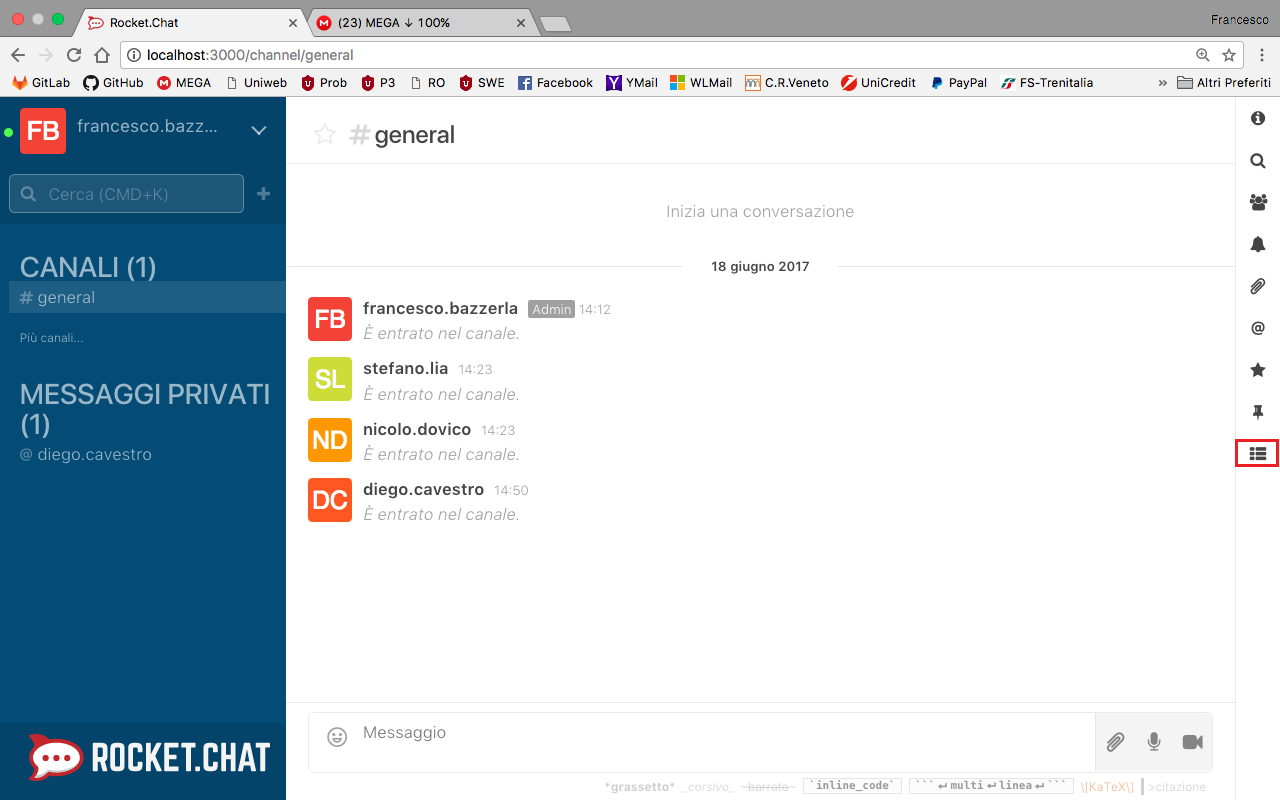
\includegraphics[width=\textwidth]{Sections/3-HowToUse/Images/button_list_create.png}
  \caption{Bubble creation button.}
\end{figure}

This will open the following screen, where you can input all the information that you want about the list, reminding that the only \textbf{required option} is the list's title.

\begin{figure}[H]
  \centering 
  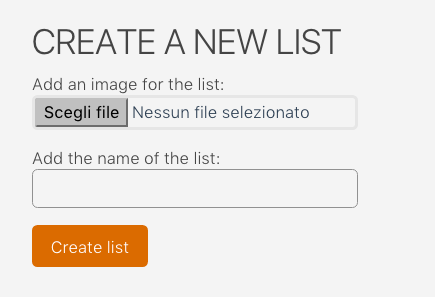
\includegraphics[width=\textwidth]{Sections/3-HowToUse/Images/list_create.png}
  \caption{Empty bubble creation input screen.}
\end{figure}

Once that all the information are input, in order to create the list just click on the \textit{"Create"} button, which will create the bubble as shown below.

\begin{figure}[H]
  \centering 
  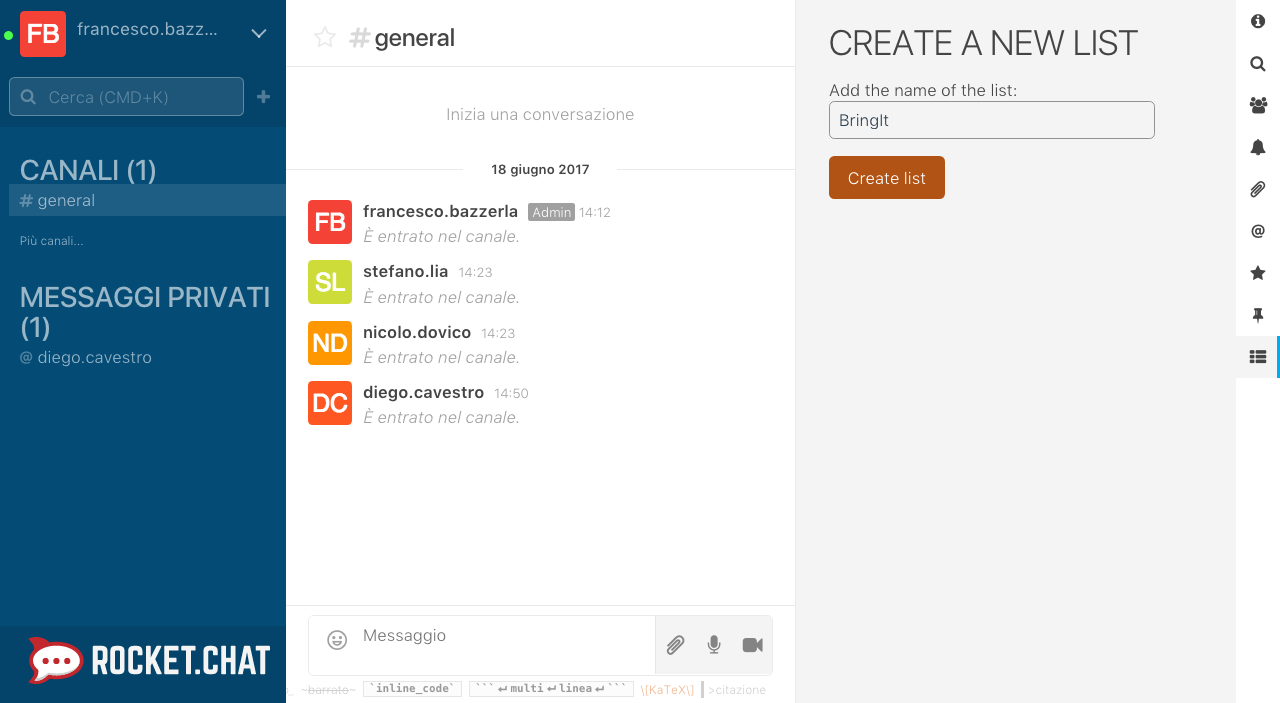
\includegraphics[width=\textwidth]{Sections/3-HowToUse/Images/list_create_filled.png}
  \caption{Filled bubble creation input screen.}
\end{figure}

% Inserire immagine della bolla creata
\begin{figure}[H]
  \centering 
  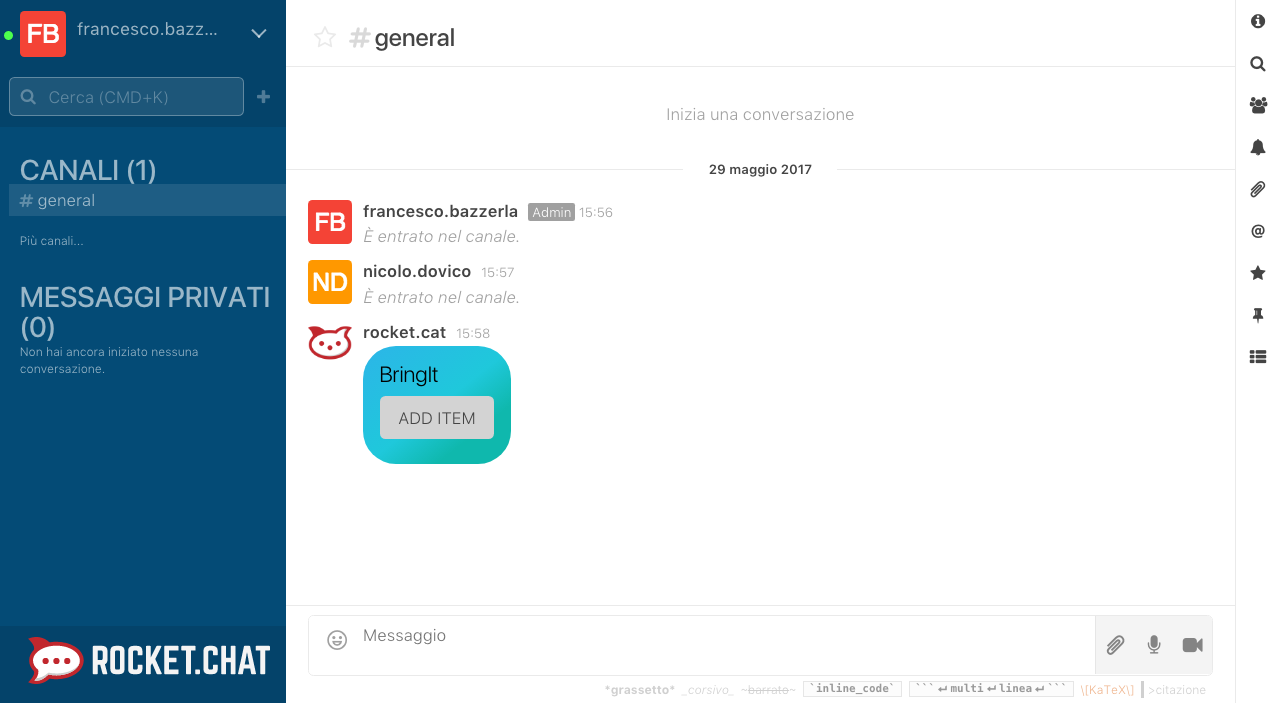
\includegraphics[width=\textwidth]{Sections/3-HowToUse/Images/bubble_empty.png}
  \caption{Created bubble which represents the list.}
\end{figure}
\newpage
\subsection{[U] Deleting a list}
In order to delete a list, hover above the bubble that represents the list, and click on the options button.

\begin{figure}[H]
  \centering 
  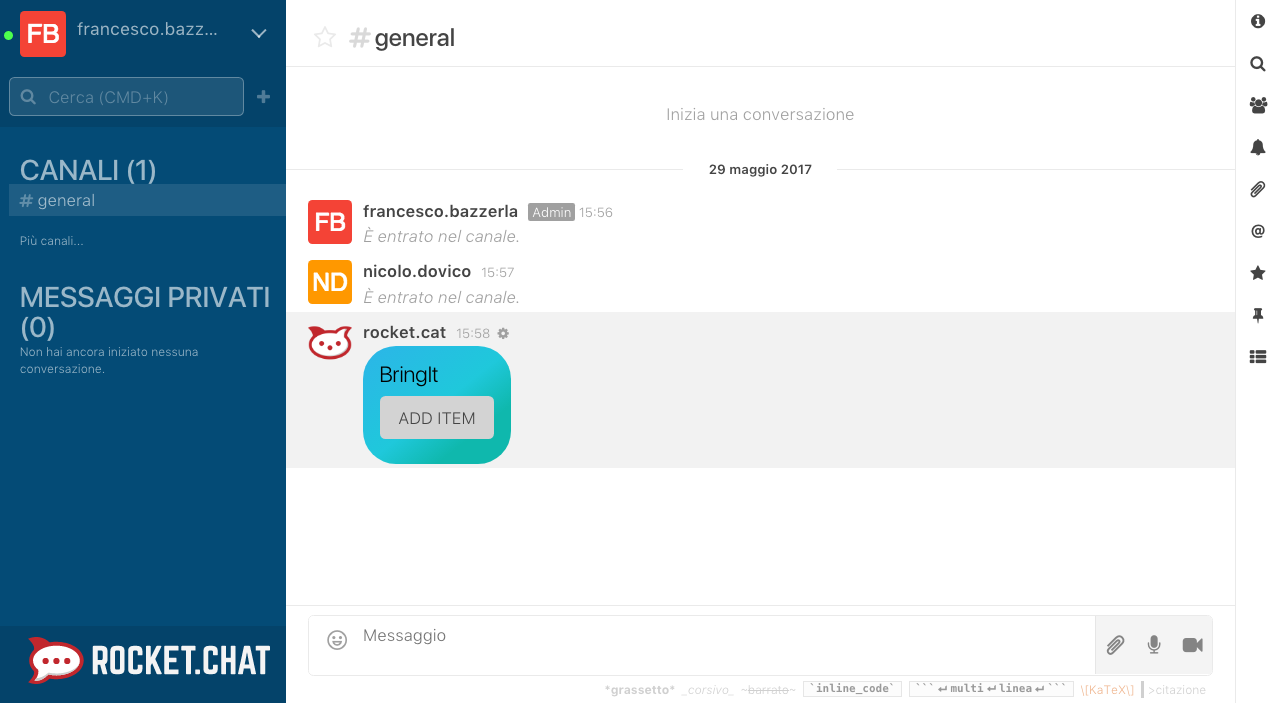
\includegraphics[width=\textwidth]{Sections/3-HowToUse/Images/bubble_options_button.png}
  \caption{Button to show the available list's actions.}
\end{figure}

From the options that appear, click on the one to delete the list, represented by an "X".

% Inserire immagine del bottone
\begin{figure}[H]
  \centering 
  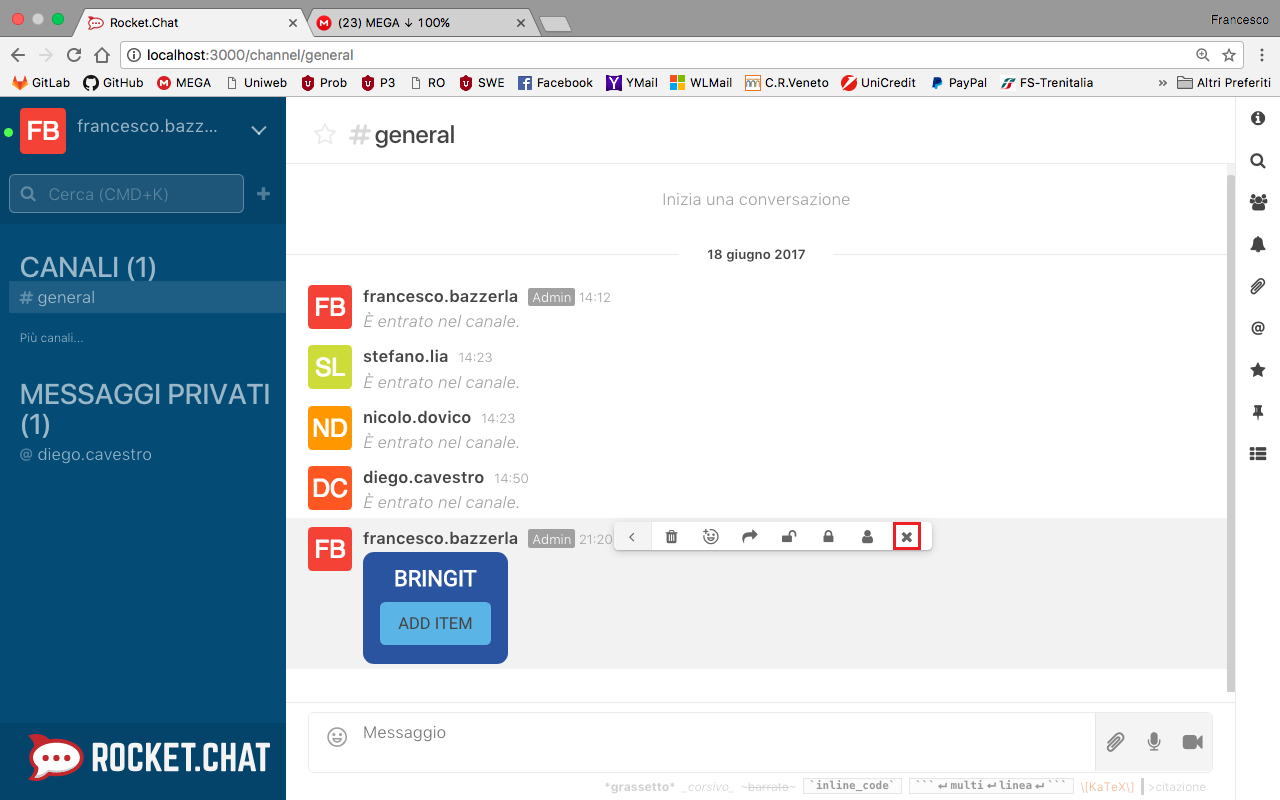
\includegraphics[width=\textwidth]{Sections/3-HowToUse/Images/bubble_option_delete.png}
  \caption{Button to delete a list.}
\end{figure}

This will open the following popup, asking you if you want to confirm the deletion.

\begin{figure}[H]
  \centering 
  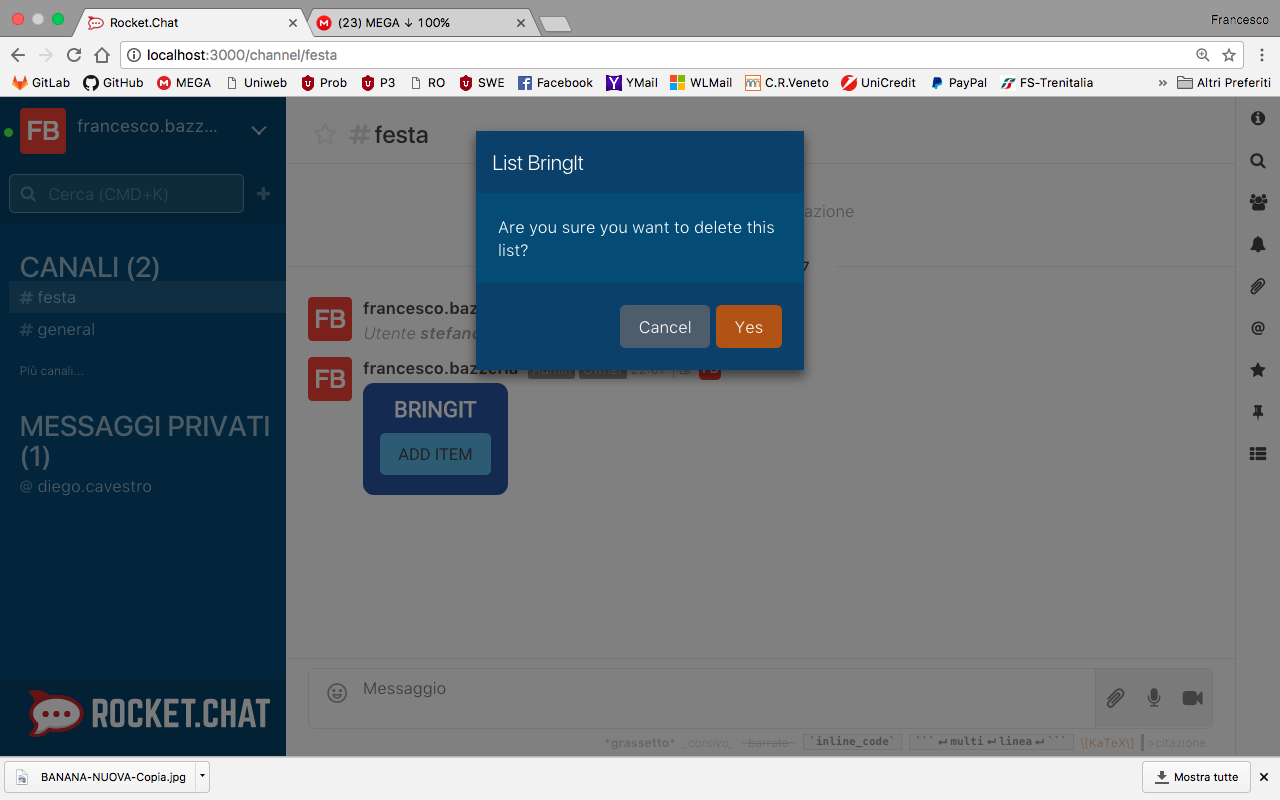
\includegraphics[width=\textwidth]{Sections/3-HowToUse/Images/popup_delete_confirm.png}
  \caption{Popup to confirm the deletion of a list.}
\end{figure}

Once you click on "Yes", the list will be deleted, showing you the popup telling that the deletion has been successful.

\begin{figure}[H]
  \centering 
  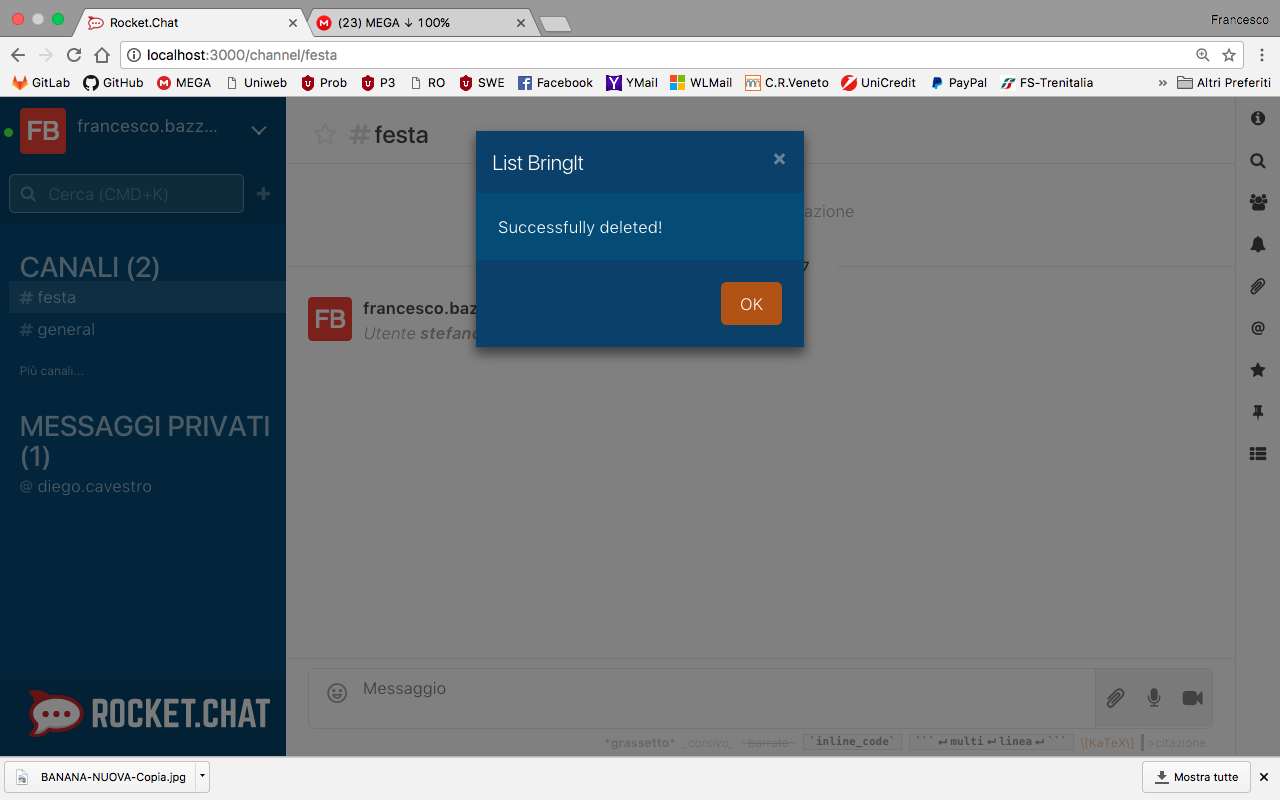
\includegraphics[width=\textwidth]{Sections/3-HowToUse/Images/popup_delete_success.png}
  \caption{Popup indicating the success of the deletion of a list.}
\end{figure}

In order to delete the bubble that represents that list, you also have to confirm the operation from the following popup that will be opened.

% Inserire immagine della bolla creata
\begin{figure}[H]
  \centering 
  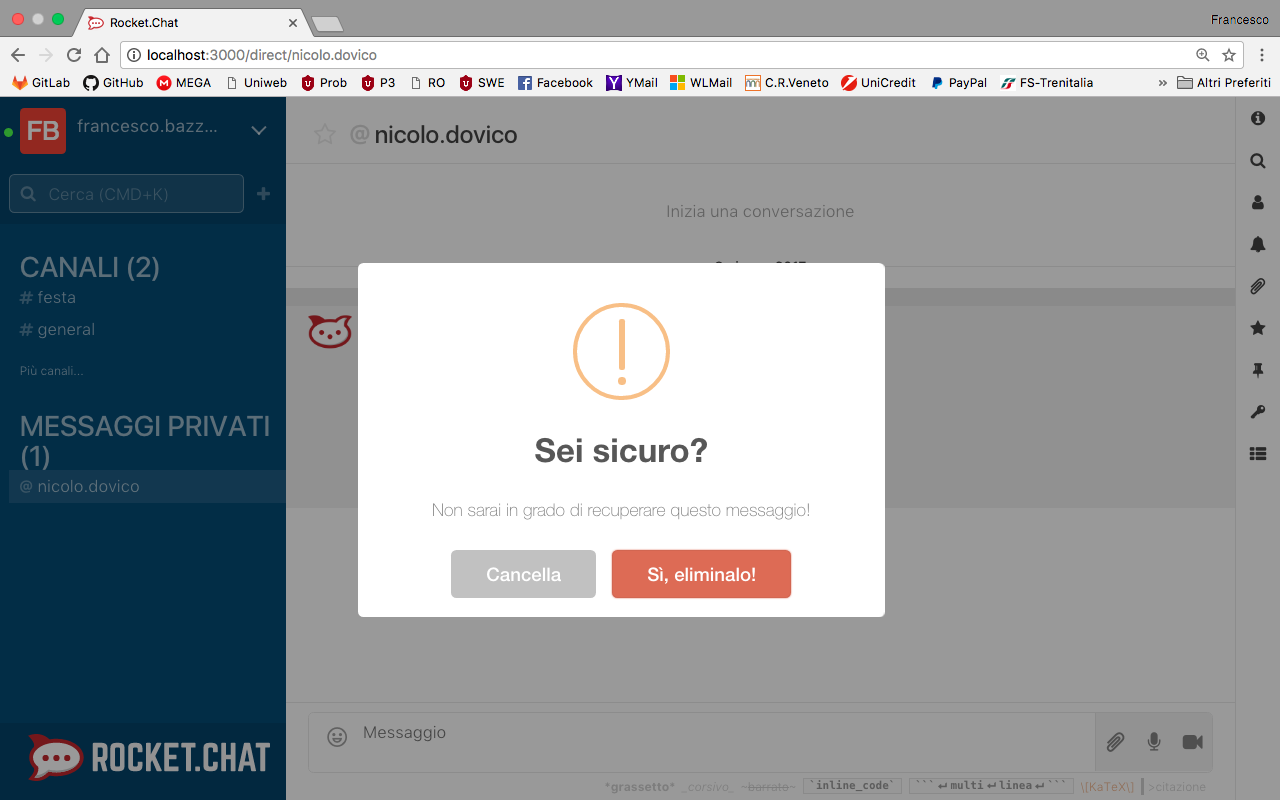
\includegraphics[width=\textwidth]{Sections/3-HowToUse/Images/popup_delete_message.png}
  \caption{Popup asking to delete the bubble representing a list.}
\end{figure}

Once that \textit{"Yes, delete it!"} will be clicked, the list will be deleted.

\newpage
\subsection{[E] Adding an item to the list}
In order to add an item to the list, just click on the proper button that is present on the bubble that represents the list itself.

% Immagine della bolla con il bottone per aggiungere un oggetto
\begin{figure}[H]
  \centering 
  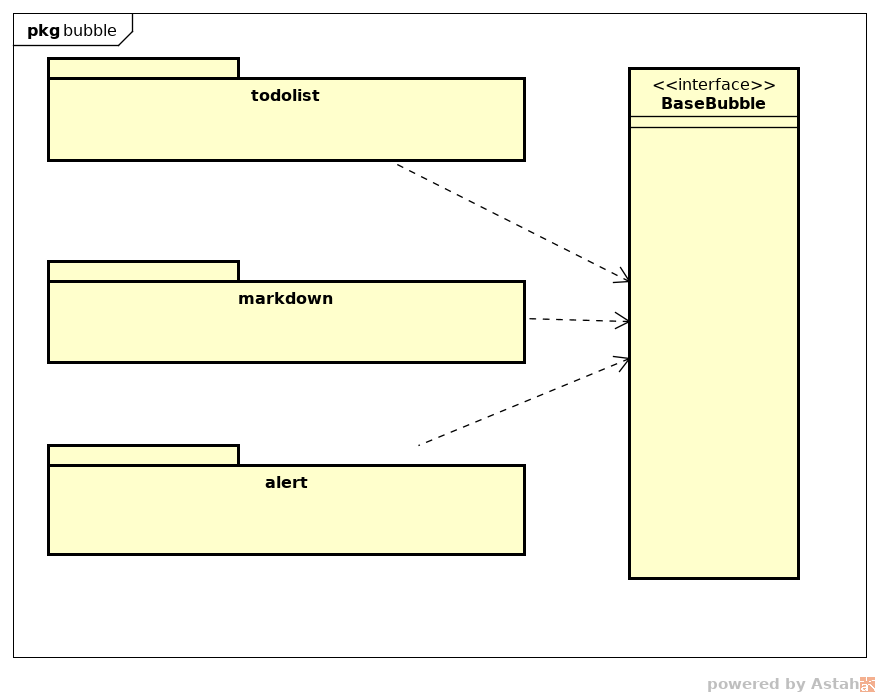
\includegraphics[scale=0.3]{Sections/3-HowToUse/Images/bubble.png}
  \caption{Bubble with the button to add an item inside.}
\end{figure}

This will open the following screen, where you can input all the information about the item that needs to be added to the list. \\

% Immagine della schermata per inserimento dati oggetto
\begin{figure}[H]
  \centering 
  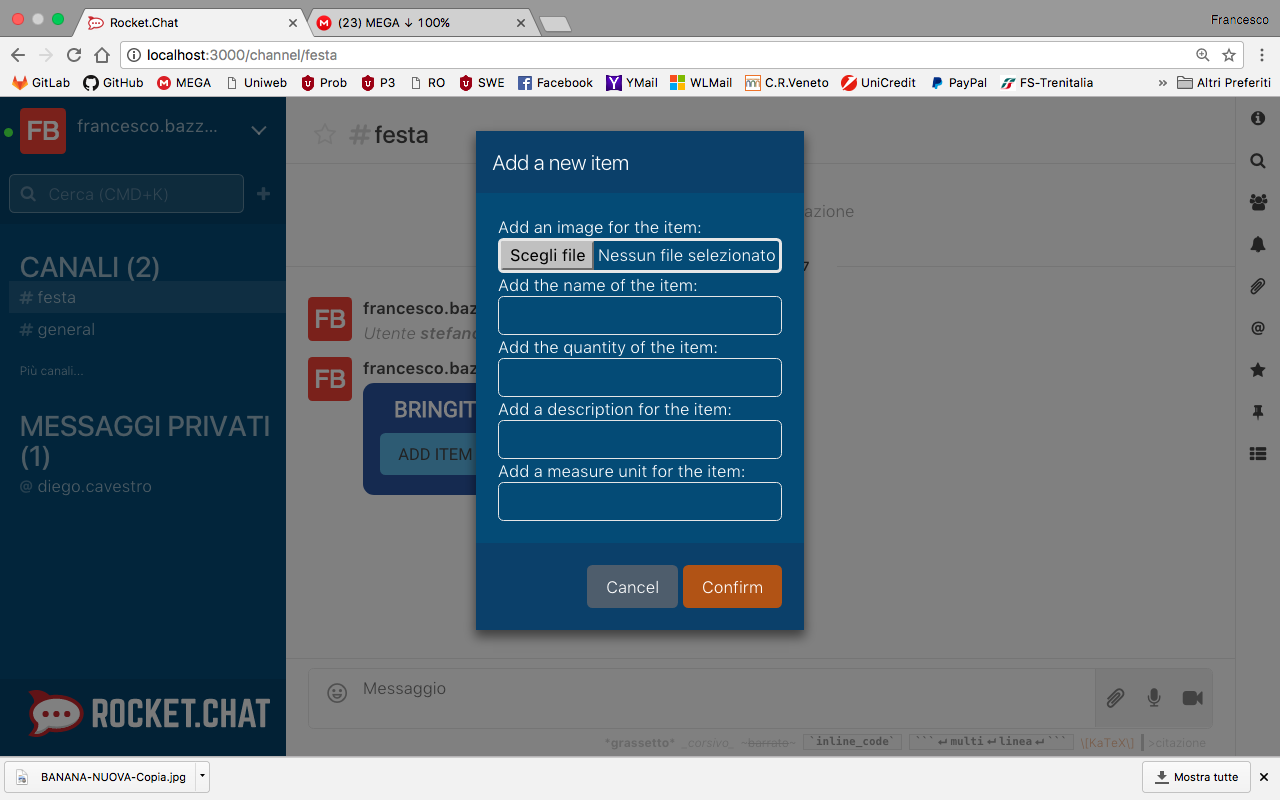
\includegraphics[scale=0.5]{Sections/3-HowToUse/Images/item_add.png}
  \caption{Item information input screen.}
\end{figure}

Once that all the data have been input, in order to add the item just click on the \textit{"Add"} button, which will add the item to the list.

% Immagine della bolla con il nuovo oggetto aggiunto
\begin{figure}[H]
  \centering 
  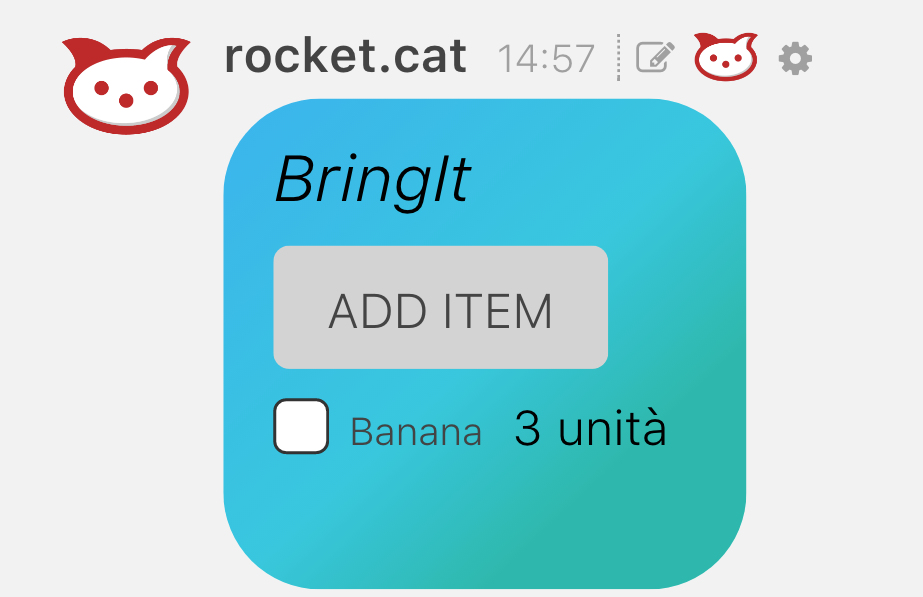
\includegraphics[scale=0.3]{Sections/3-HowToUse/Images/bubble_with_item.png}
  \caption{Bubble with the new item added.}
\end{figure}
\subsection{[E] Editing an item *}
In order to edit the information of an item inside the list, just long click the item that you want to edit, opening the following screen.

% Immagine della schermata di edit dei dati di un oggetto
\begin{figure}[H]
  \centering 
  
\includegraphics[width=\textwidth]{Sections/3-HowToUse/Images/example.jpeg}
  \caption{Item information editing screen.}
\end{figure}

Once you have modified all the information that you want, just click on the \textit{"Save"} button, which will save the edits you have performed.

% Immagine della bolla con l'oggetto modificato
\begin{figure}[H]
  \centering 
  
\includegraphics[width=\textwidth]{Sections/3-HowToUse/Images/example.jpeg}
  \caption{Bubble with the edited item inside.}
\end{figure}
\newpage
\subsection{[E] Removing an item from the list}
In order to remove an item from the list, just long click on the item that you want to remove. This will open the following popup showing the item's details.

\begin{figure}[H]
  \centering 
  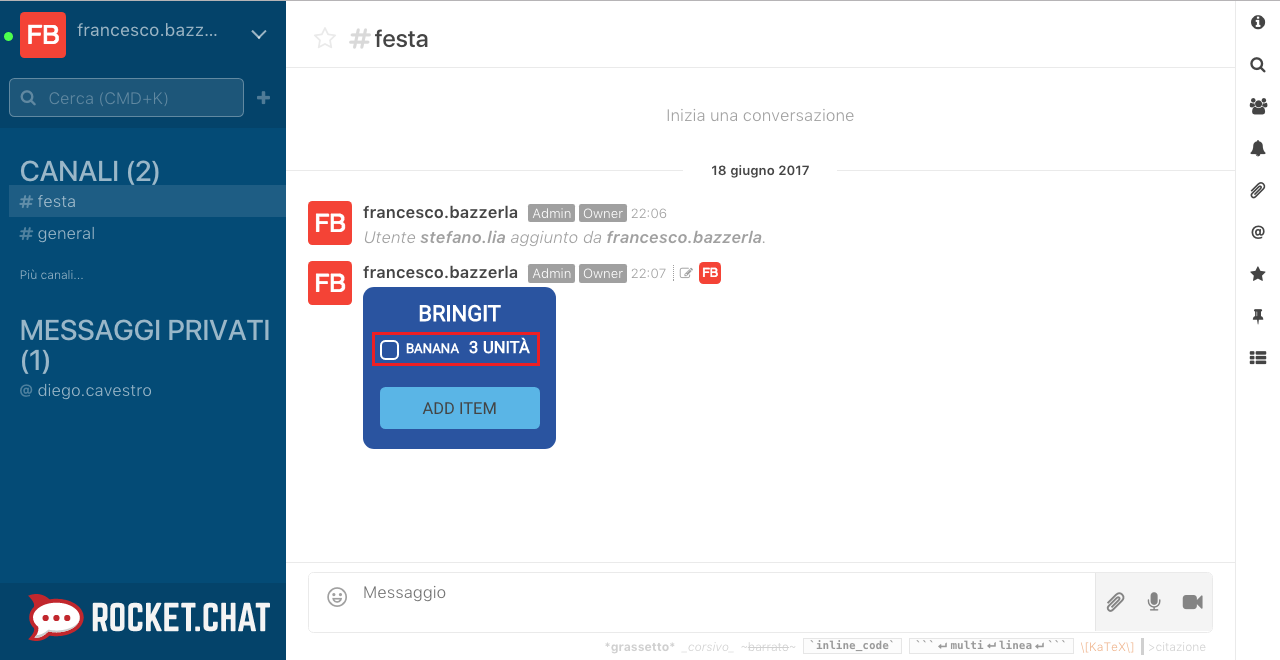
\includegraphics[width=\textwidth]{Sections/3-HowToUse/Images/bubble_item_to_delete.png}
  \caption{Popup showing the details of an item.}
\end{figure}

\begin{figure}[H]
  \centering 
  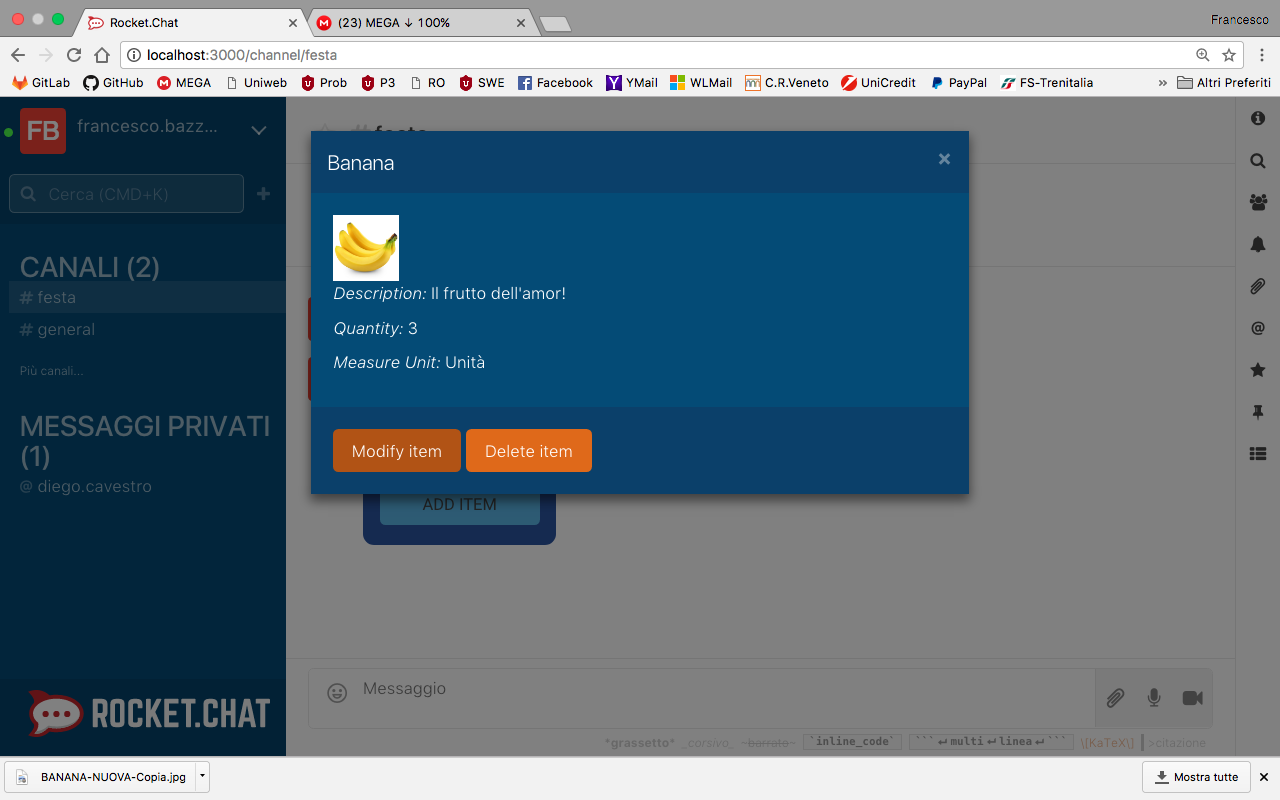
\includegraphics[width=\textwidth]{Sections/3-HowToUse/Images/item_details.png}
  \caption{Popup showing the details of an item.}
\end{figure}

To delete the item, just click on the \textit{"Delete"} button.

\begin{figure}[H]
  \centering 
  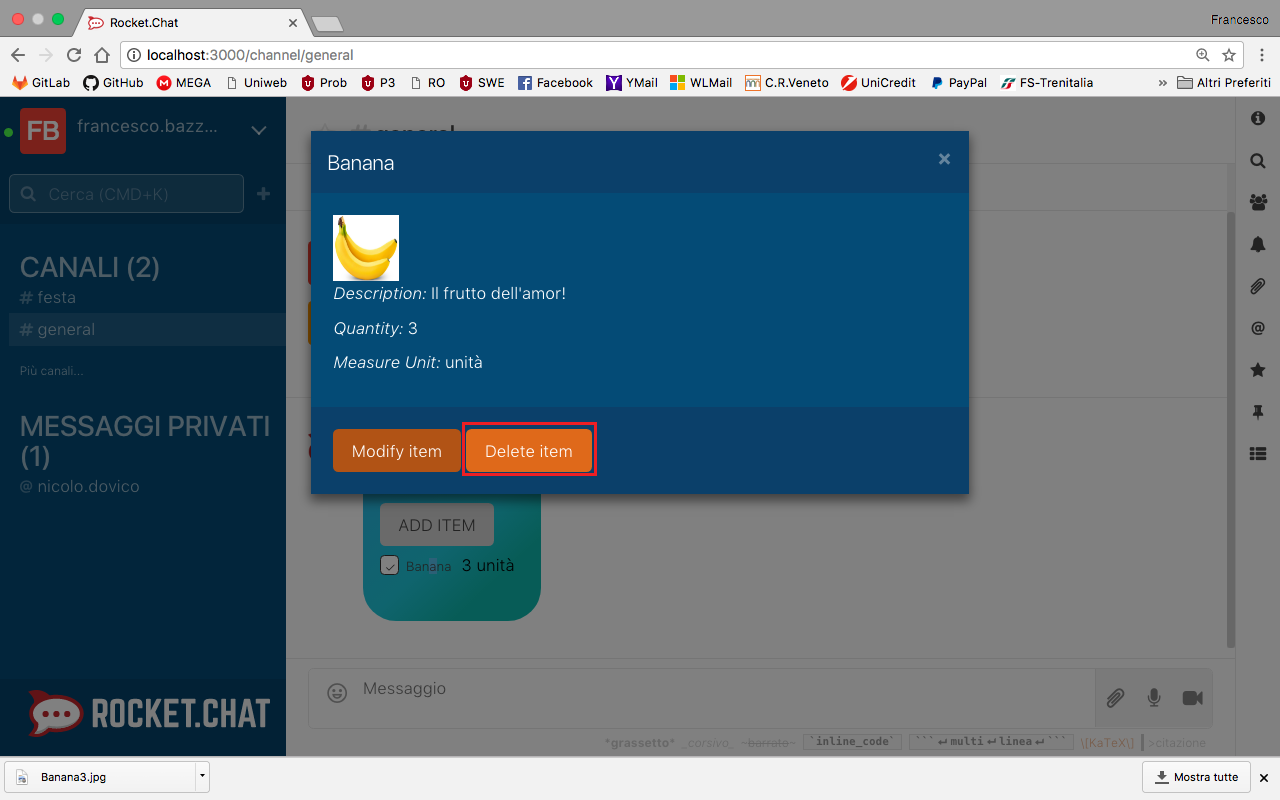
\includegraphics[width=\textwidth]{Sections/3-HowToUse/Images/popup_item_delete.png}
  \caption{Button to delete an item from a list.}
\end{figure}

\begin{figure}[H]
  \centering 
  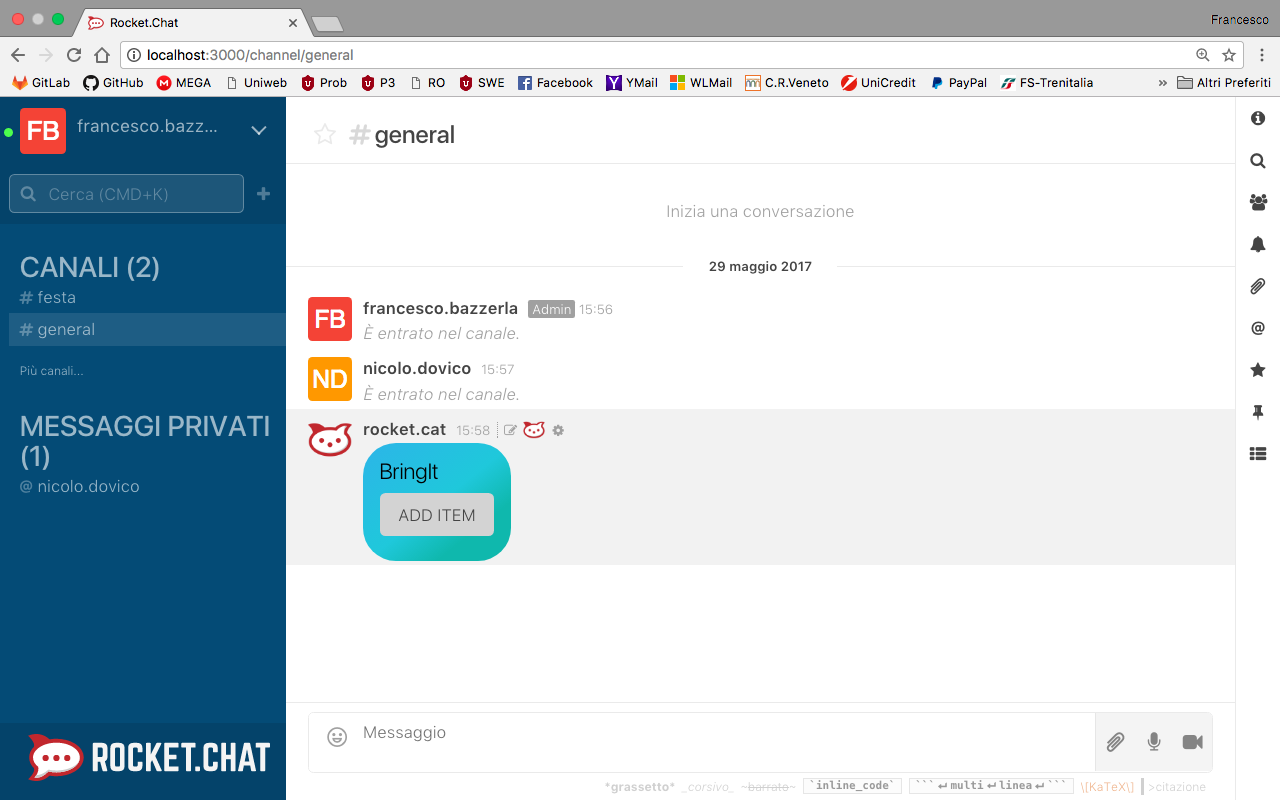
\includegraphics[width=\textwidth]{Sections/3-HowToUse/Images/bubble_item_deleted.png}
  \caption{Bubble with the deleted item.}
\end{figure}

\newpage
\subsection{[C] Sharing a list with a group}
In order to share a list with a group, hover on top of the \termine{bubble} that represents the list and click on the gear icon.

\begin{figure}[H]
  \centering 
  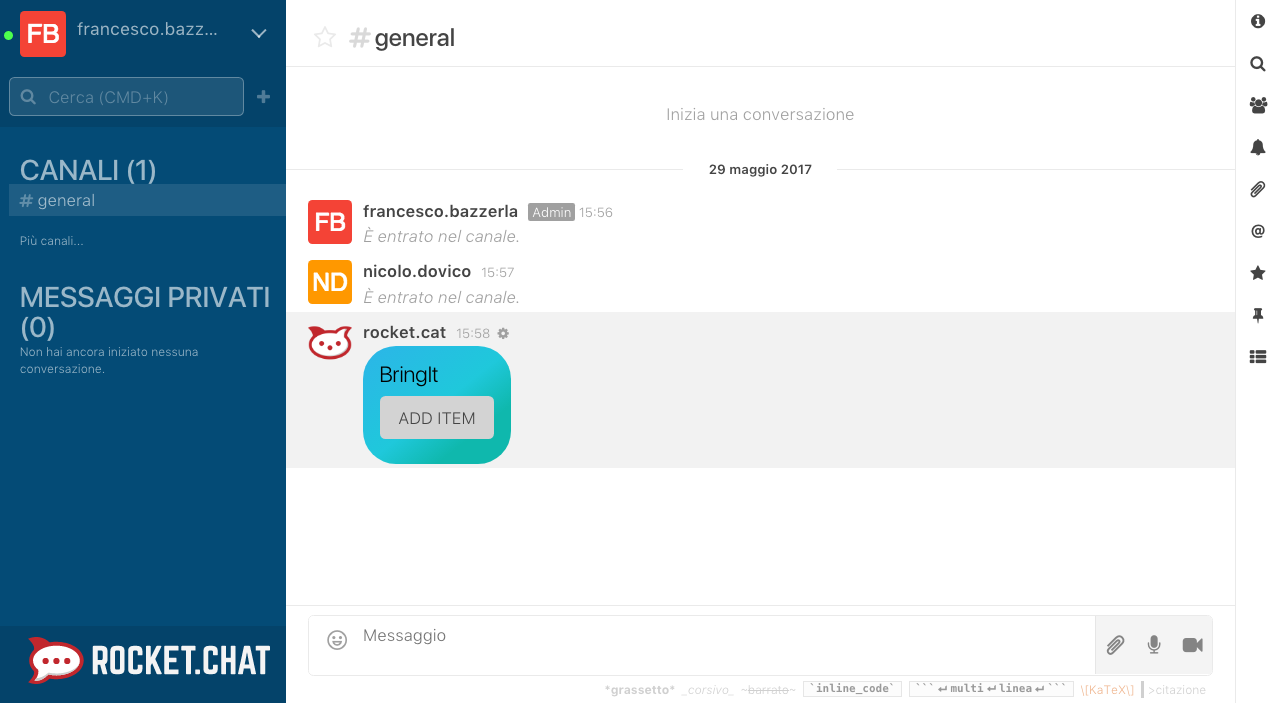
\includegraphics[width=\textwidth]{Sections/3-HowToUse/Images/bubble_options_button.png}
  \caption{Button to show the available list's actions.}
\end{figure}

From the various options that are available, click on the one with the sharing icon.

\begin{figure}[H]
  \centering 
  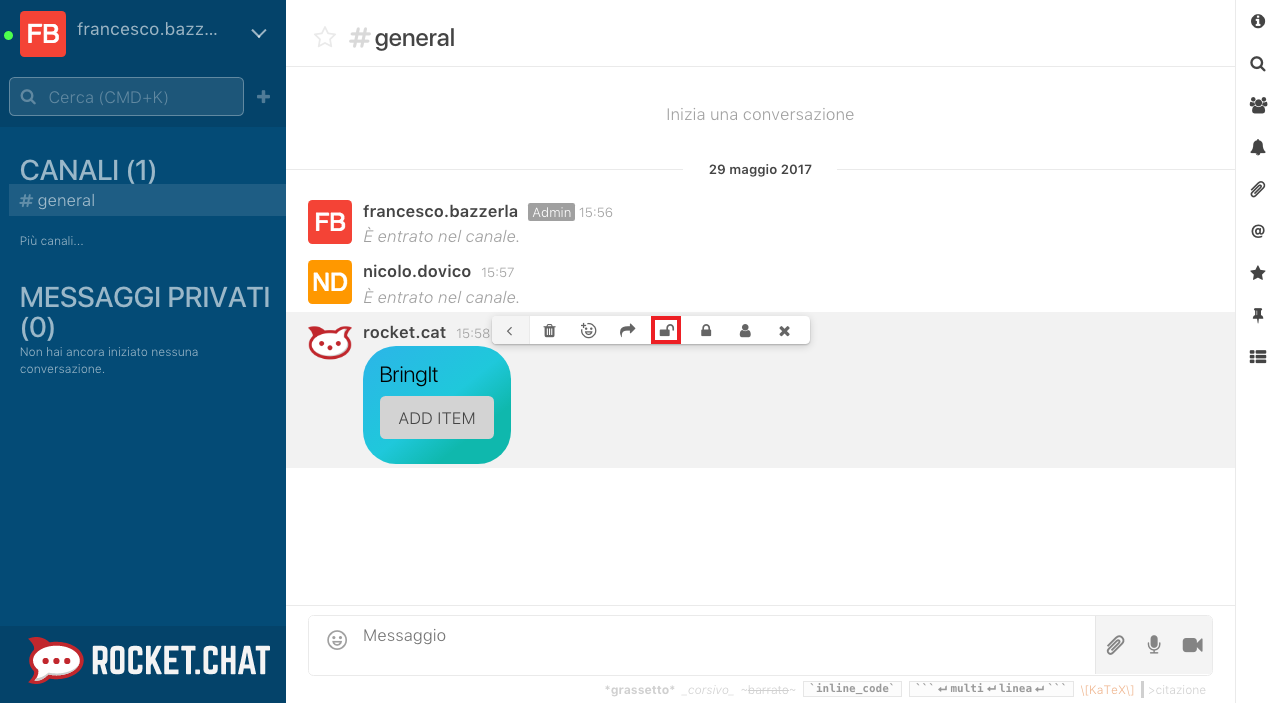
\includegraphics[width=\textwidth]{Sections/3-HowToUse/Images/bubble_option_share_group.png}
  \caption{Button to share the list with a specific group.}
\end{figure}

Once that the option has been clicked, the following popup will appear, showing the list of all the group that the list can be shared to.

\begin{figure}[H]
  \centering 
  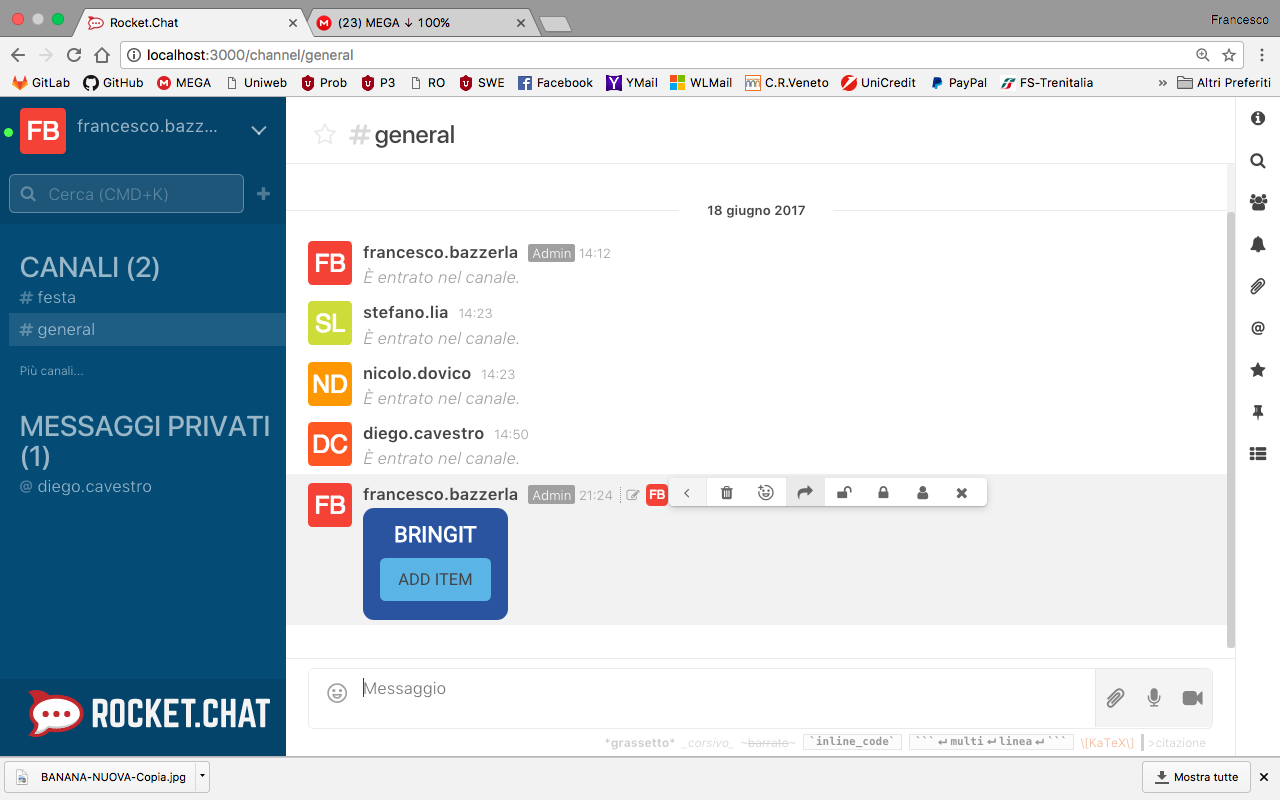
\includegraphics[width=\textwidth]{Sections/3-HowToUse/Images/share_group_channel.png}
  \caption{Popup showing the list of all the groups to which is possible sharing a list.}
\end{figure}

Now, select the group you want share the list with and then click on \textit{"Share"}. \\
This will open a new popup, letting you choose to which user you want to grant the \textbf{editor} permission. Once you have chose to which users to grant the permissions, click on \textit{"Ok"}.

\begin{figure}[H]
  \centering 
  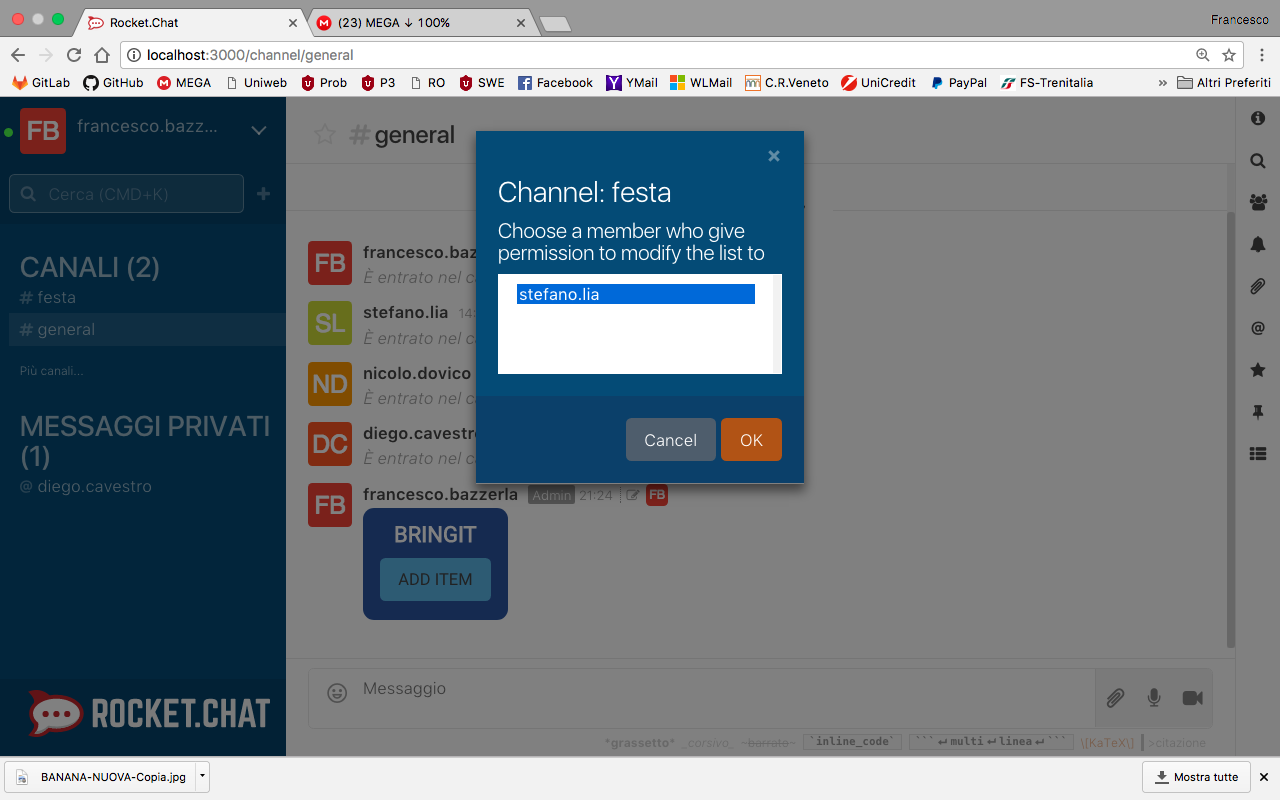
\includegraphics[width=\textwidth]{Sections/3-HowToUse/Images/share_group_user.png}
  \caption{Popup to grant the editor permission to users inside the group.}
\end{figure}

Note that, if there are no users you can share the list with, an error will be shown.

\begin{figure}[H]
  \centering 
  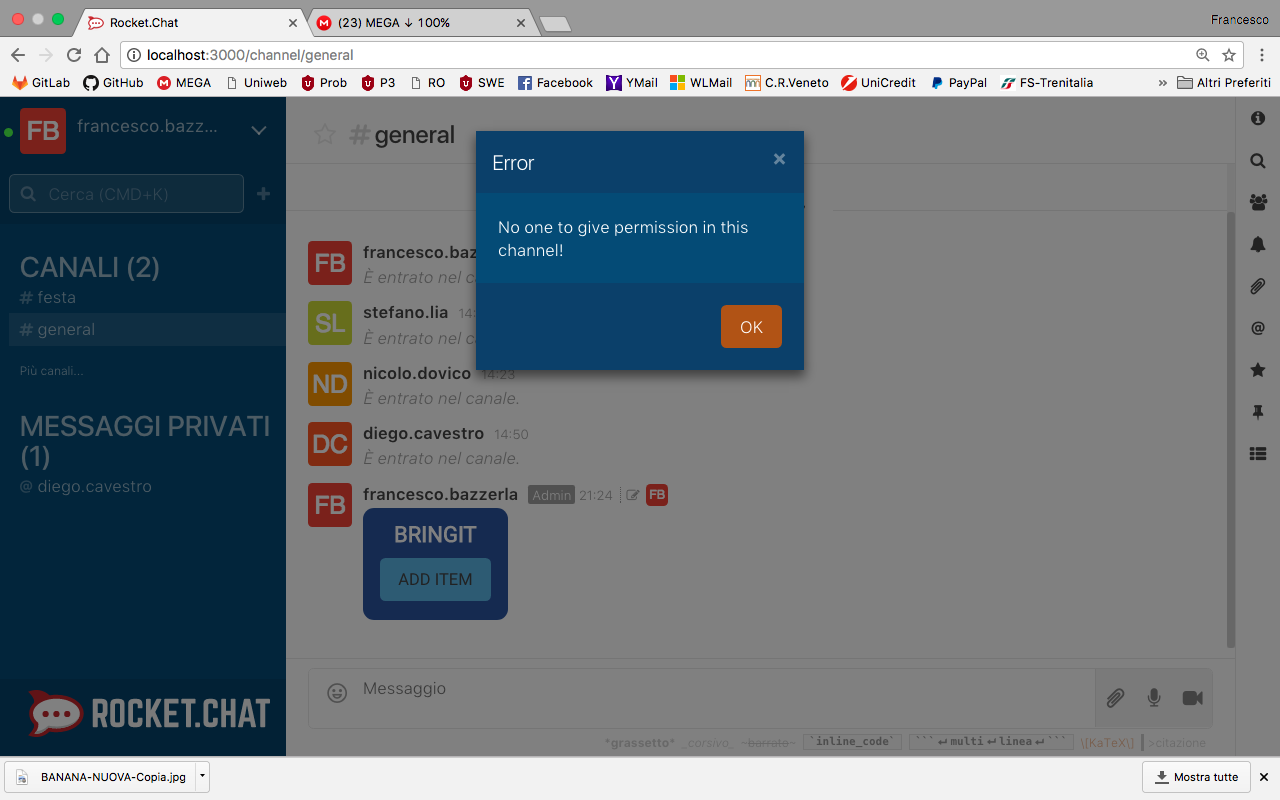
\includegraphics[width=\textwidth]{Sections/3-HowToUse/Images/popup_permission_give_error.png}
  \caption{Error shown if there are no users it's possible to share the list with.}
\end{figure}

Once that the sharing has been completed successfully, a message will be sent inside the proper channel


\begin{figure}[H]
  \centering 
  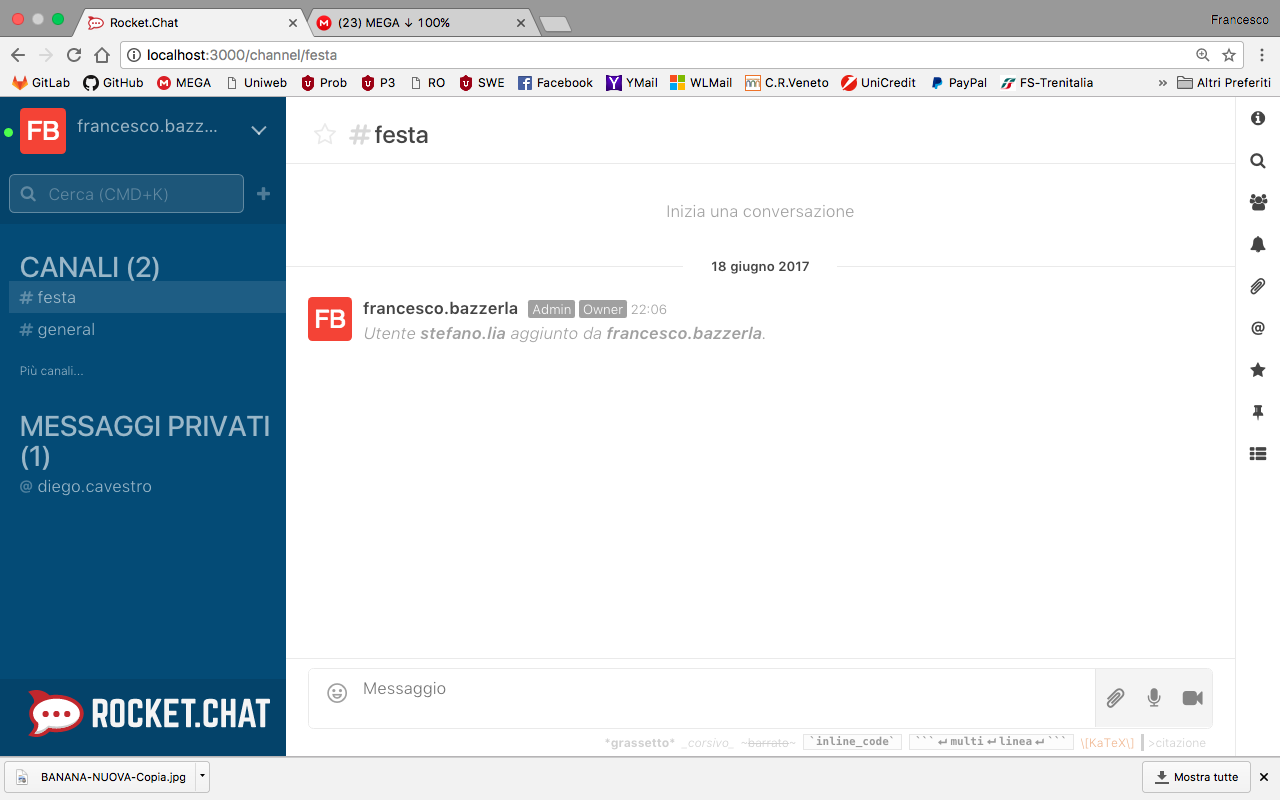
\includegraphics[width=\textwidth]{Sections/3-HowToUse/Images/share_group_before.png}
  \caption{Channel before the sharing of the list.}
\end{figure}

\begin{figure}[H]
  \centering 
  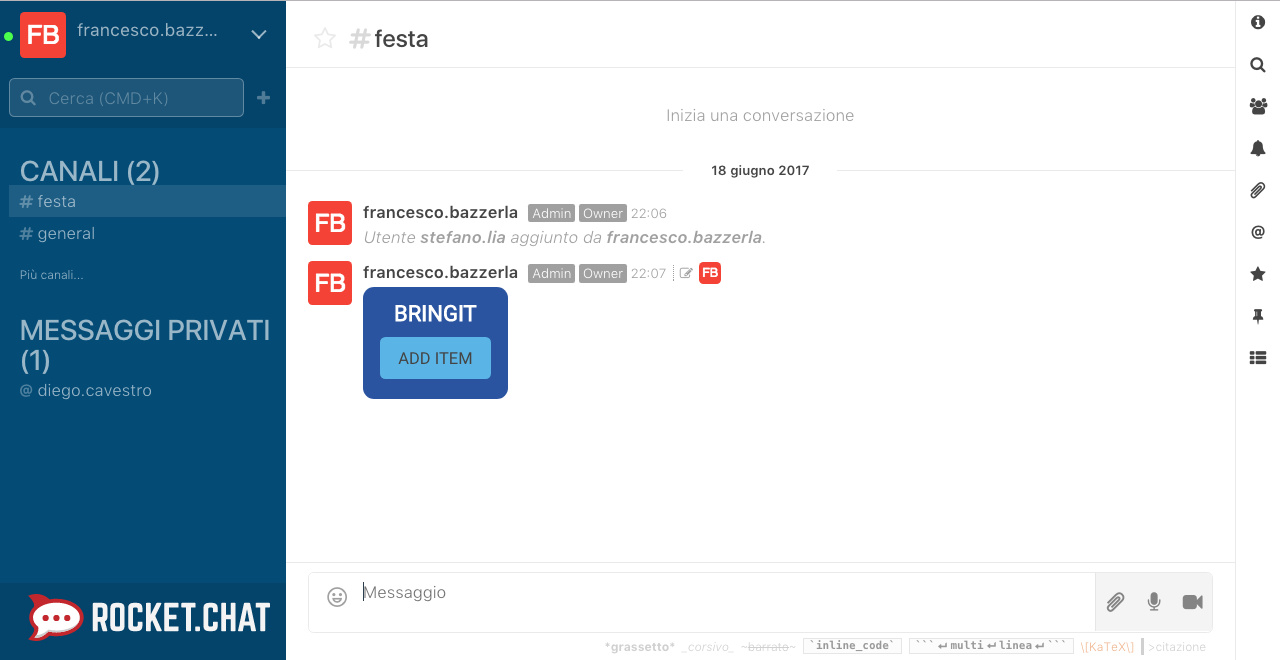
\includegraphics[width=\textwidth]{Sections/3-HowToUse/Images/share_group_after.png}
  \caption{Channel after the sharing of the list.}
\end{figure}
\newpage
\subsection{[C] Sharing a list with a user}
In order to share a list with a user, hover on top of the \termine{bubble} that represents the list and click on the gear icon.

\begin{figure}[H]
  \centering 
  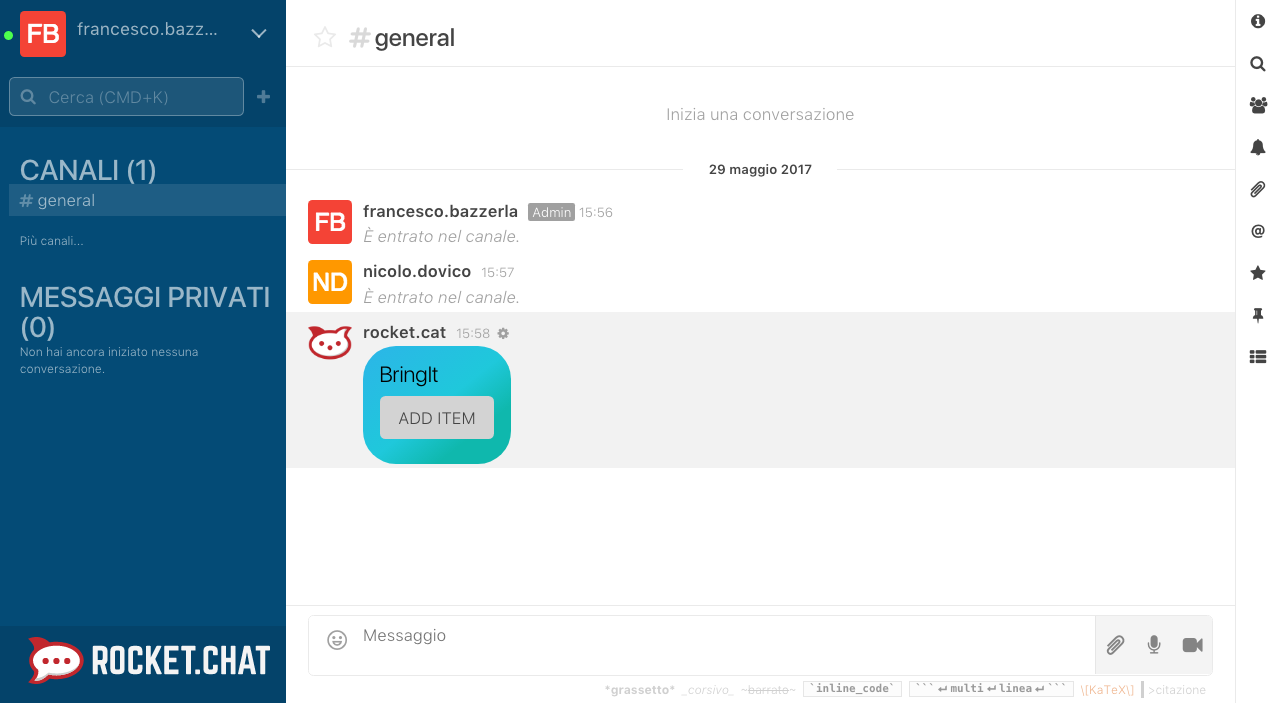
\includegraphics[width=\textwidth]{Sections/3-HowToUse/Images/bubble_options_button.png}
  \caption{Button to show the available list's actions.}
\end{figure}

From the various options that are available, click on the one with the user icon.

\begin{figure}[H]
  \centering 
  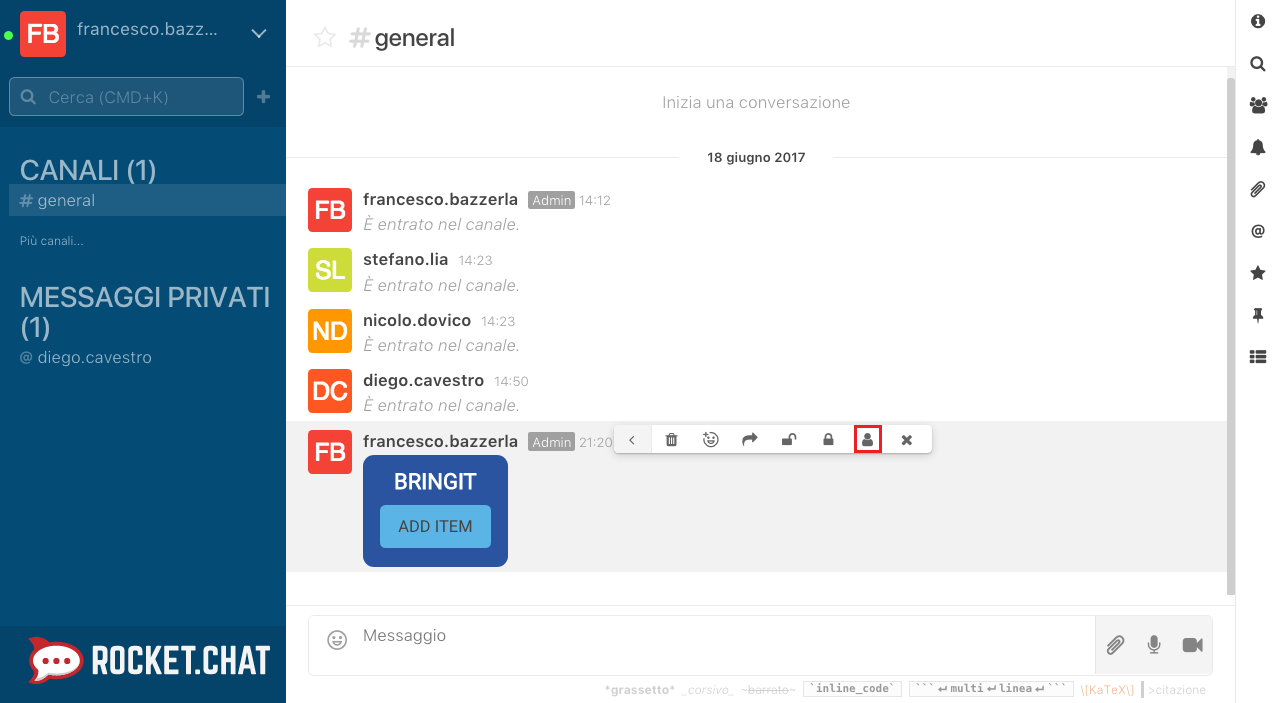
\includegraphics[width=\textwidth]{Sections/3-HowToUse/Images/bubble_option_share_user.png}
  \caption{Button to share the list with a specific user.}
\end{figure}

Once that the option has been clicked, the following popup will appear, showing the list of all the item that the list can be shared to.

\begin{figure}[H]
  \centering 
  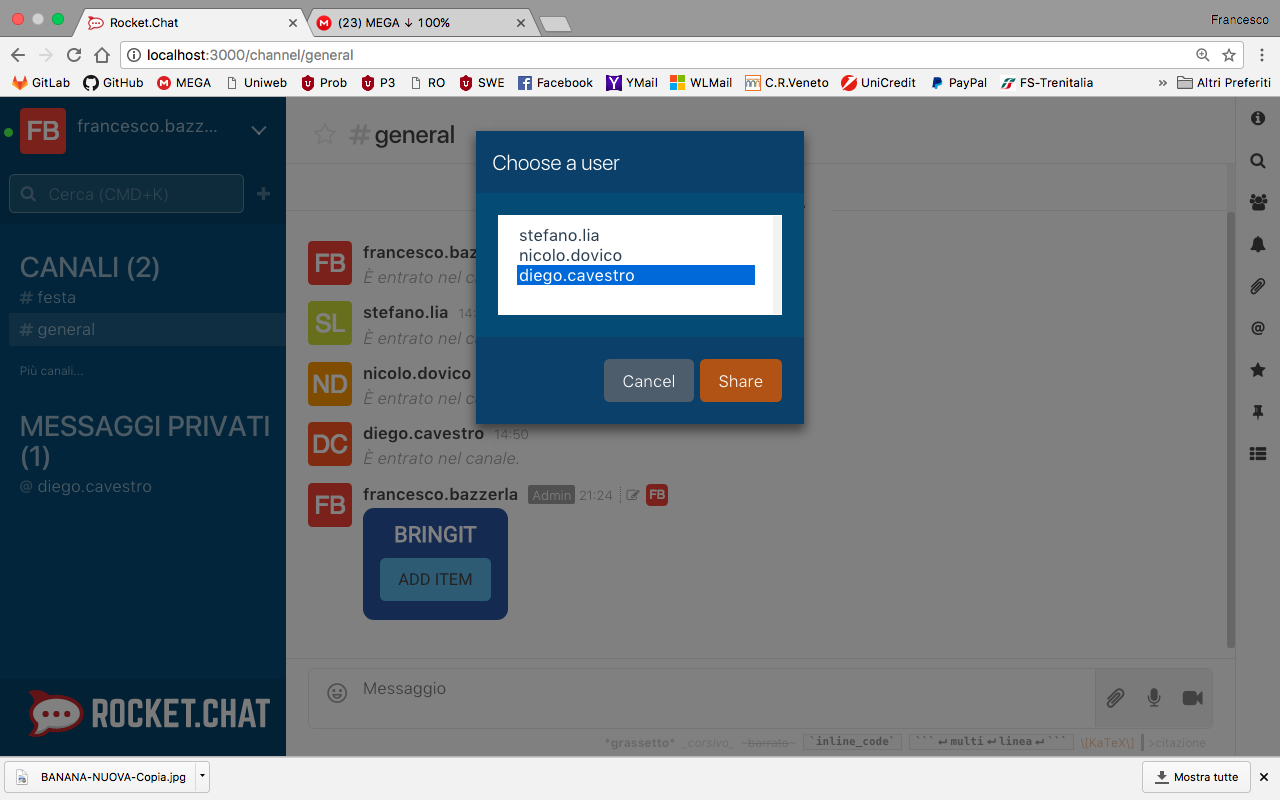
\includegraphics[width=\textwidth]{Sections/3-HowToUse/Images/popup_share_user.png}
  \caption{Popup showing the list of all the users to which is possible sharing a list.}
\end{figure}

Now, select the user you want share the list with and then click on \textit{"Share"}. \\
This will open the following popup, asking you to confirm the sharing action.

\begin{figure}[H]
  \centering 
  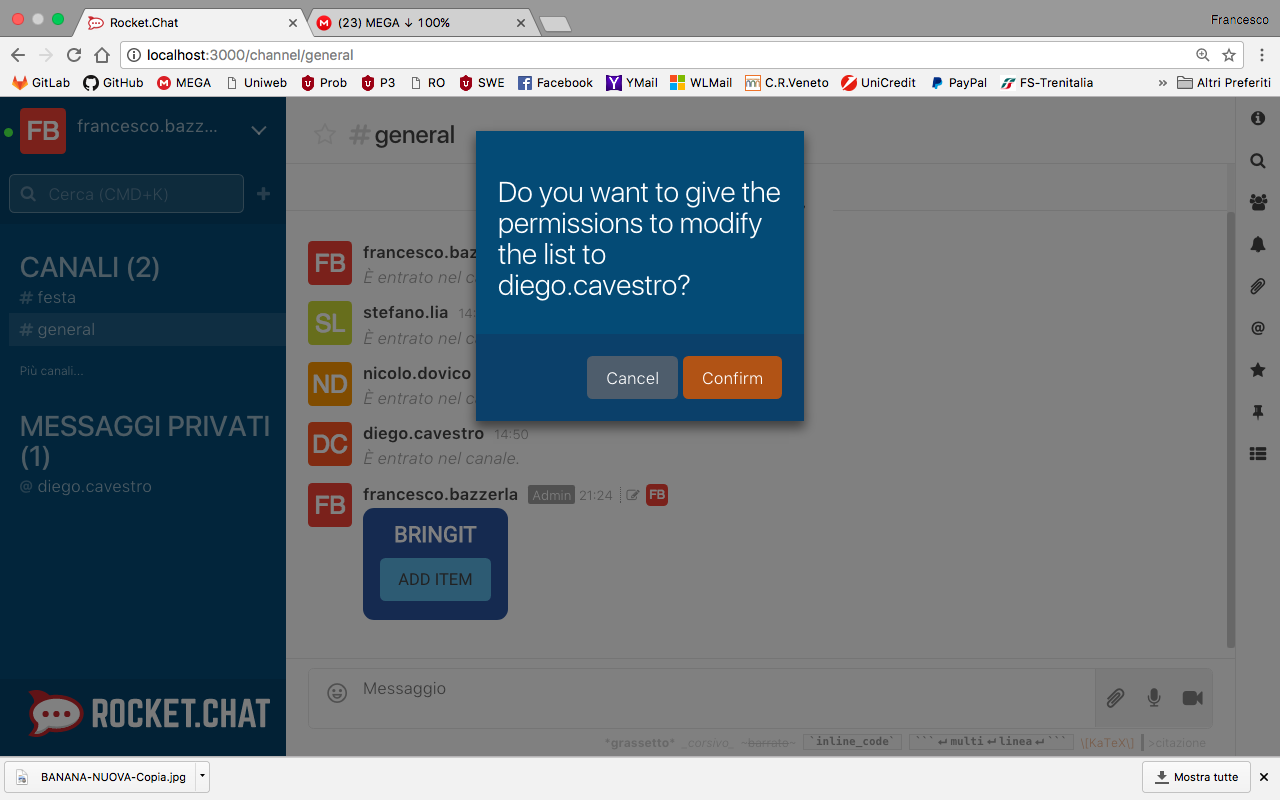
\includegraphics[width=\textwidth]{Sections/3-HowToUse/Images/popup_share_user_confirm.png}
  \caption{Popup to confirm the action to share the list with the selected user.}
\end{figure}

Once you have confirmed the sharing, the bubble will be sent inside the private chat with the user.

\begin{figure}[H]
  \centering 
  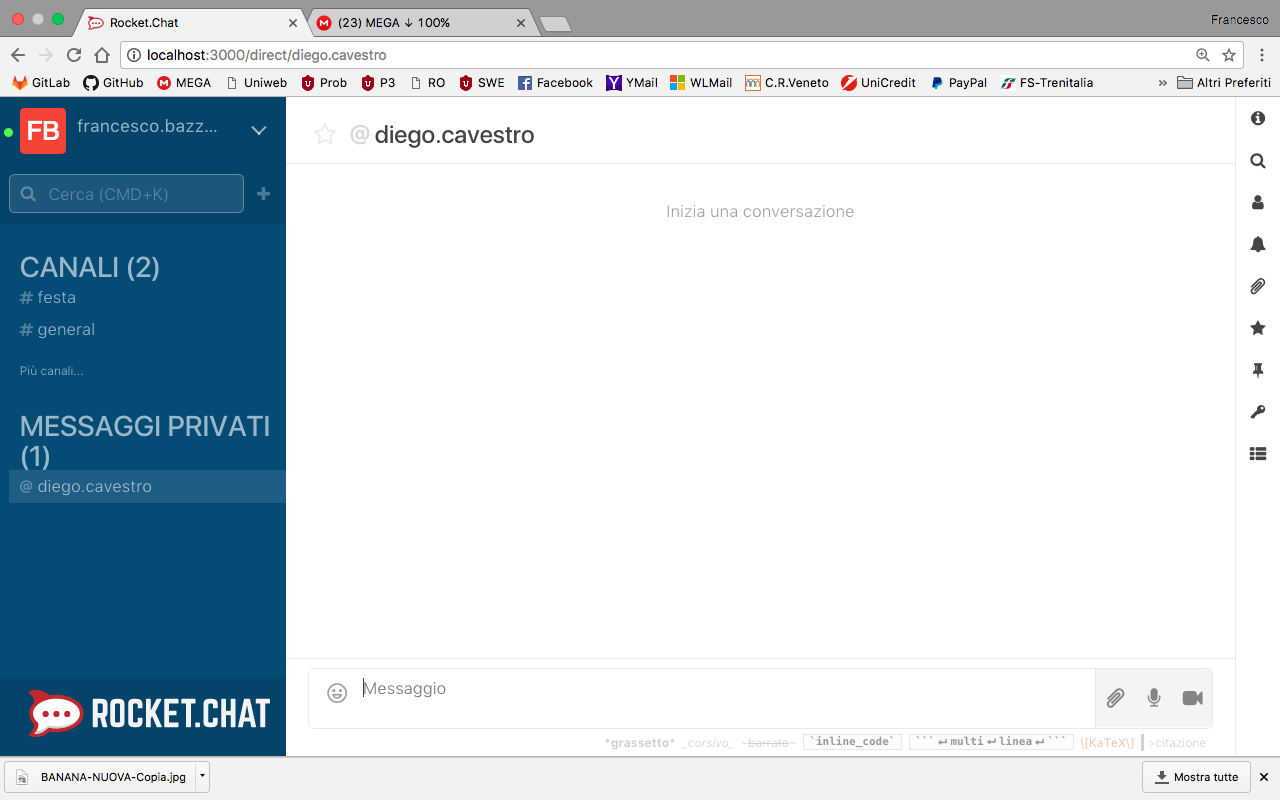
\includegraphics[width=\textwidth]{Sections/3-HowToUse/Images/share_user_before.png}
  \caption{Private chat with a user before sharing the list.}
\end{figure}

\begin{figure}[H]
  \centering 
  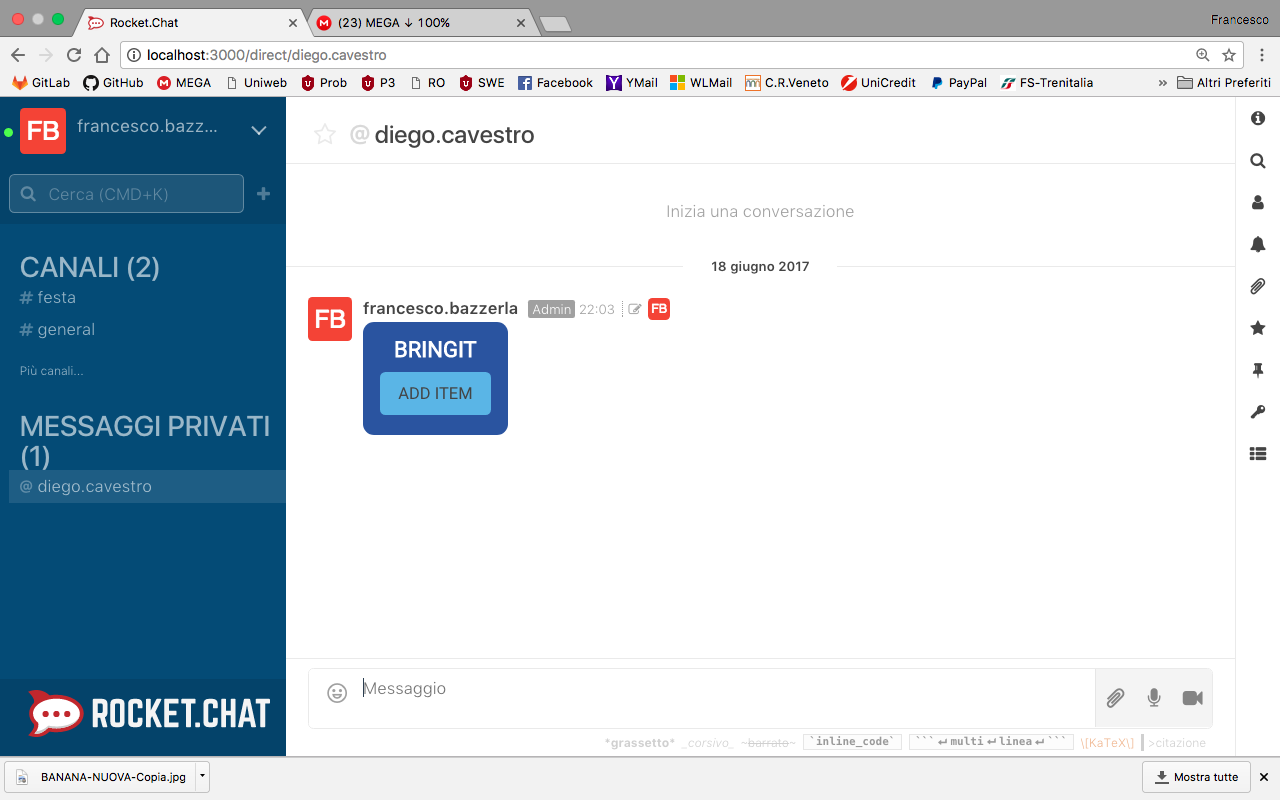
\includegraphics[width=\textwidth]{Sections/3-HowToUse/Images/share_user_after.png}
  \caption{Private chat with a user after sharing the list.}
\end{figure}




\newpage
\subsection{[C] Giving editing permissions to a user}
To add a user from the list of people that have access to the list, just hover above the bubble, and click on the options button.

\begin{figure}[H]
  \centering 
  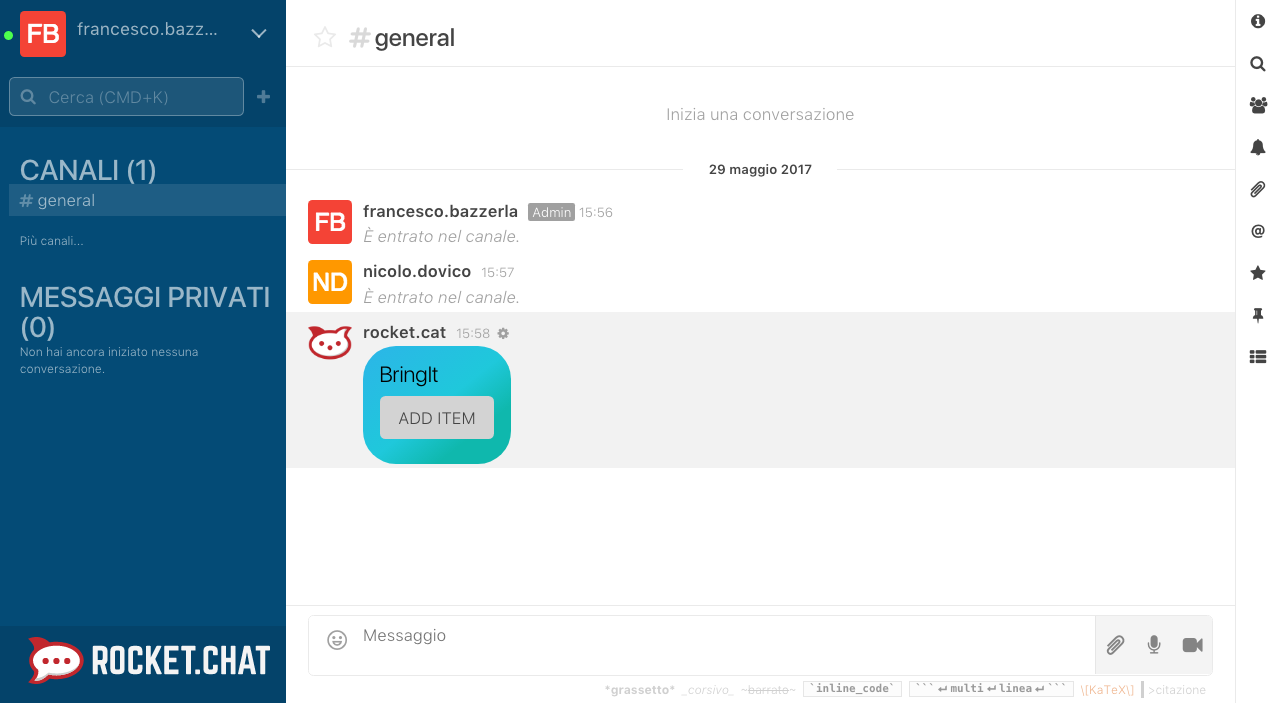
\includegraphics[width=\textwidth]{Sections/3-HowToUse/Images/bubble_options_button.png}
  \caption{Button to show the available list's actions.}
\end{figure}

Select then the button to add the permission to a user.

\begin{figure}[H]
  \centering 
  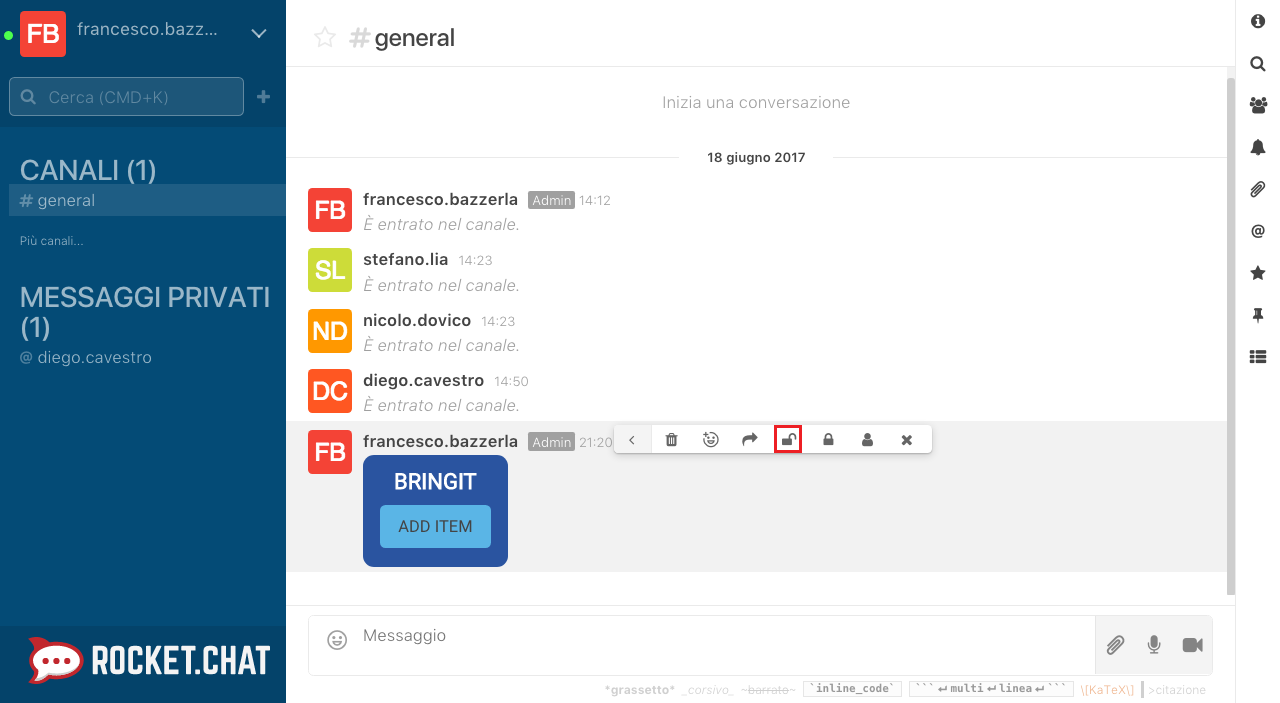
\includegraphics[width=\textwidth]{Sections/3-HowToUse/Images/bubble_option_permission_give.png}
  \caption{Button to remove the permissions of a user.}
\end{figure}

From the popup that opens, select the user(s) you want to add the permission to, and then click on "Ok".

\begin{figure}[H]
  \centering 
  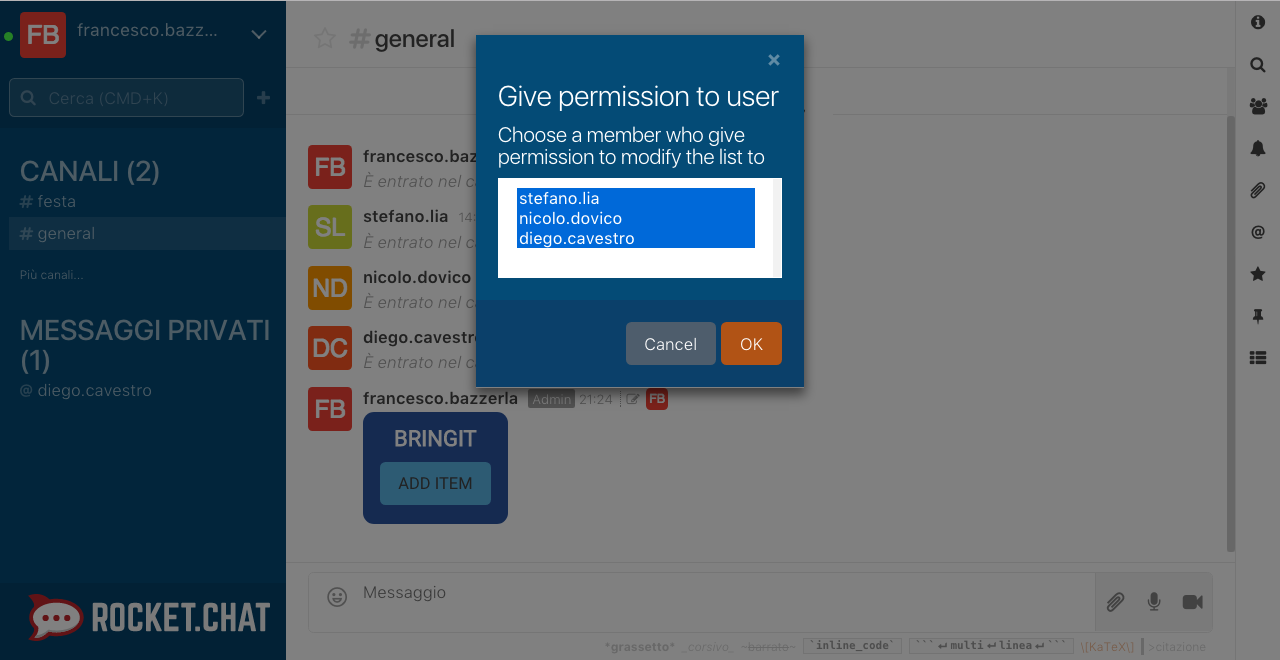
\includegraphics[width=\textwidth]{Sections/3-HowToUse/Images/popup_permission_give.png}
  \caption{Popup to remove the permissions of a user.}
\end{figure}

Note that, if there are no users from which you can remove the permissions, an error will be shown.

\begin{figure}[H]
  \centering 
  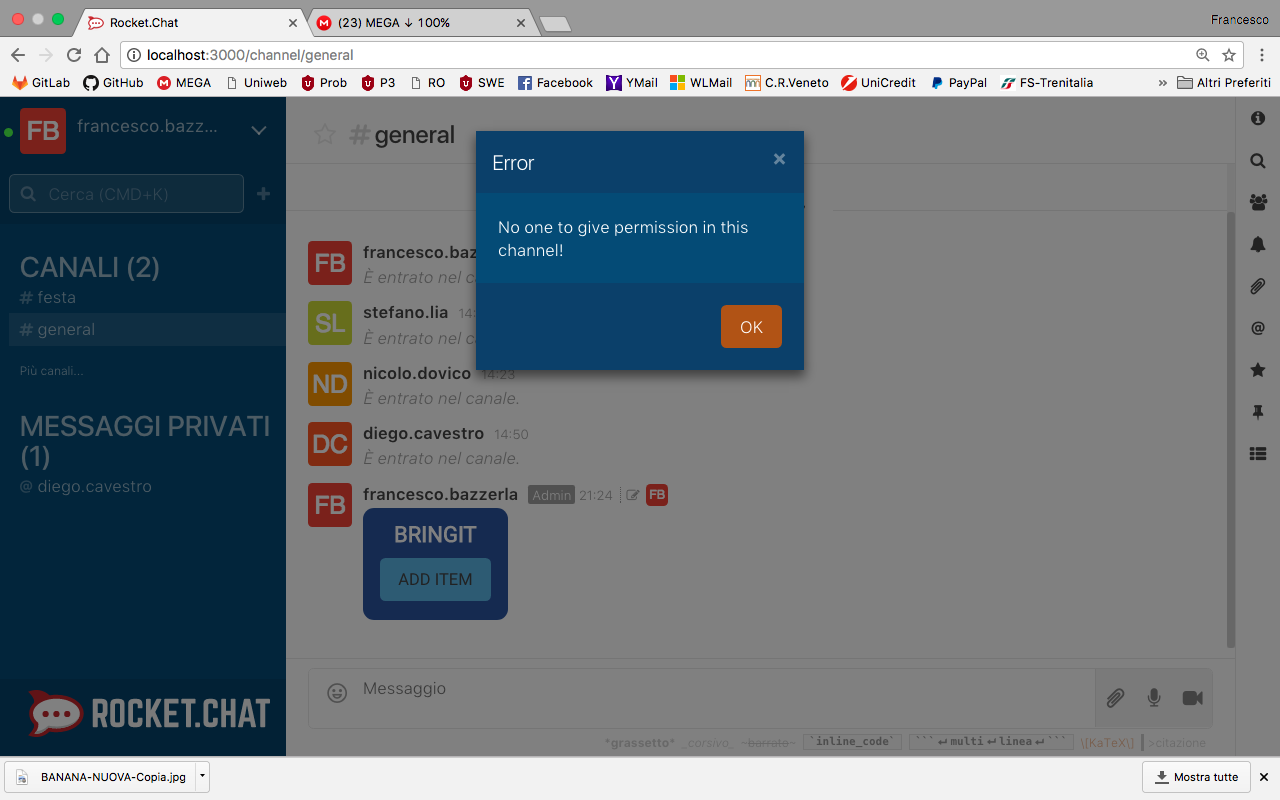
\includegraphics[width=\textwidth]{Sections/3-HowToUse/Images/popup_permission_give_error.png}
  \caption{Error shown if there are no people you can remove the permissions from.}
\end{figure}
\newpage
\subsection{[C] Removing a user}
To remove a user from the list of people that have access to the list, just hover above the bubble, and click on the options button.

\begin{figure}[H]
  \centering 
  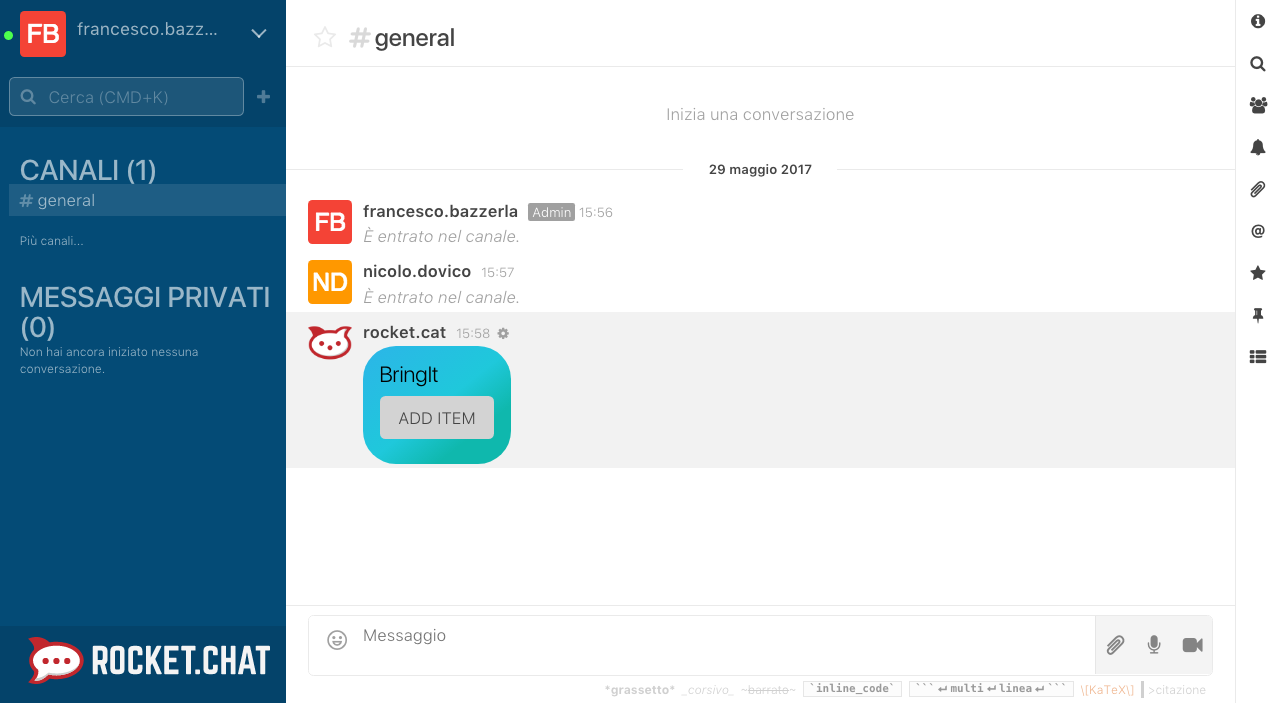
\includegraphics[width=\textwidth]{Sections/3-HowToUse/Images/bubble_options_button.png}
  \caption{Button to show the available list's actions.}
\end{figure}

Select then the button to remove the permissions of a user.

\begin{figure}[H]
  \centering 
  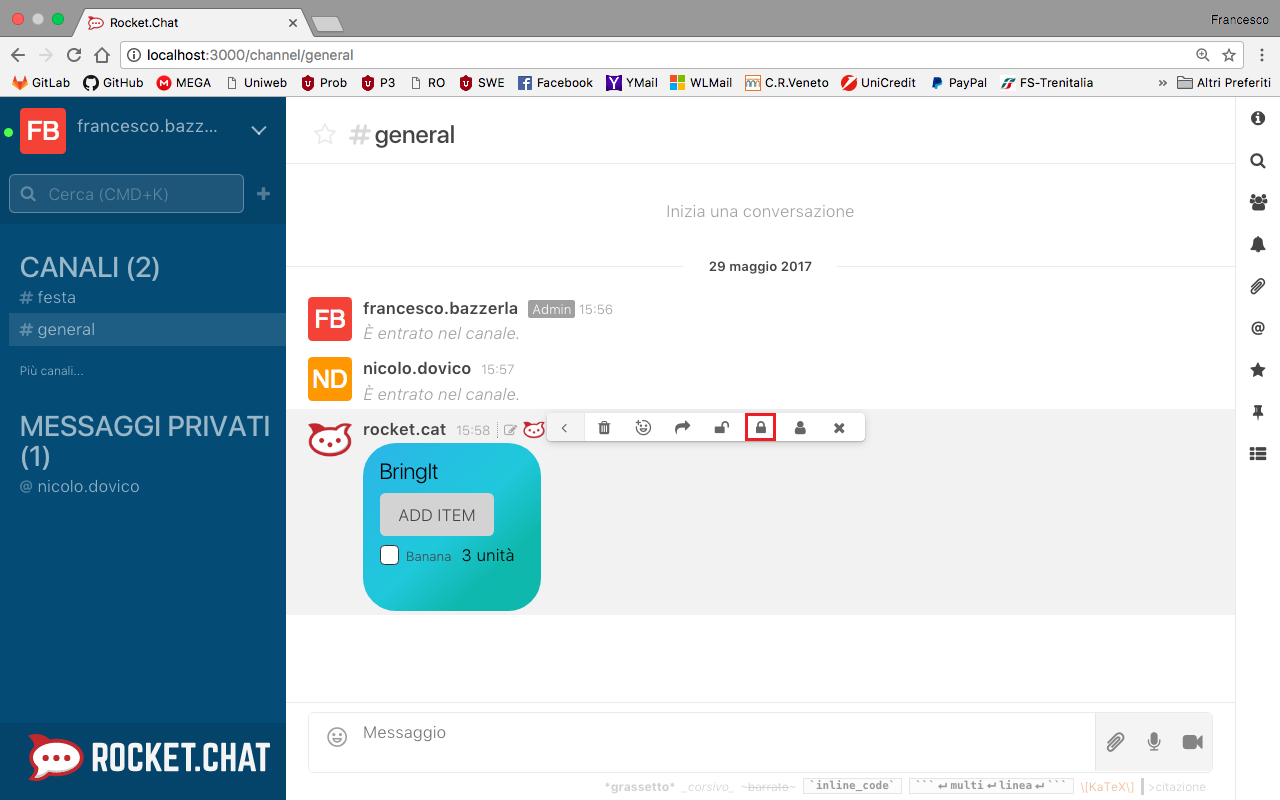
\includegraphics[width=\textwidth]{Sections/3-HowToUse/Images/bubble_option_remove.png}
  \caption{Button to remove the permissions of a user.}
\end{figure}

From the popup that opens, select the user(s) you want to remove the permission from, and then click on "Ok".

\begin{figure}[H]
  \centering 
  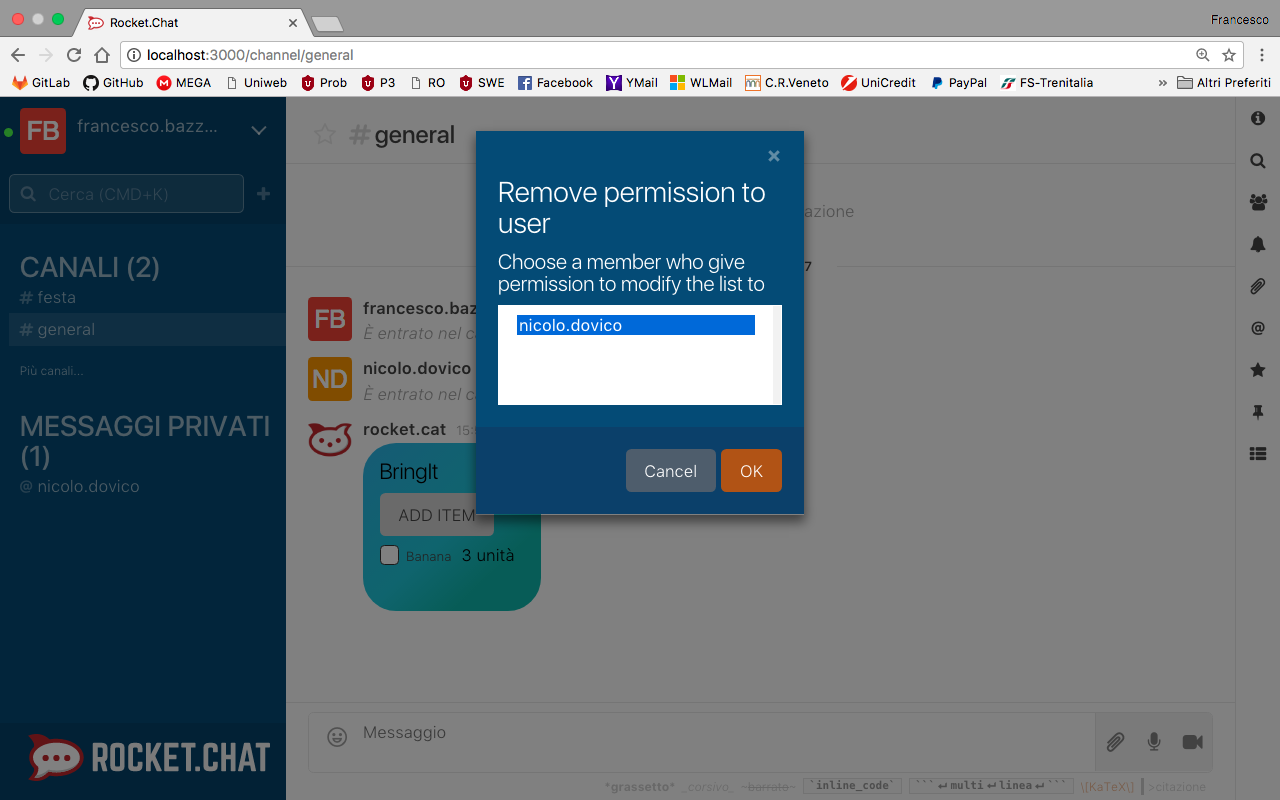
\includegraphics[width=\textwidth]{Sections/3-HowToUse/Images/permission_remove.png}
  \caption{Popup to remove the permissions of a user.}
\end{figure}

Note that, if there are no users from which you can remove the permissions, an error will be shown.

\begin{figure}[H]
  \centering 
  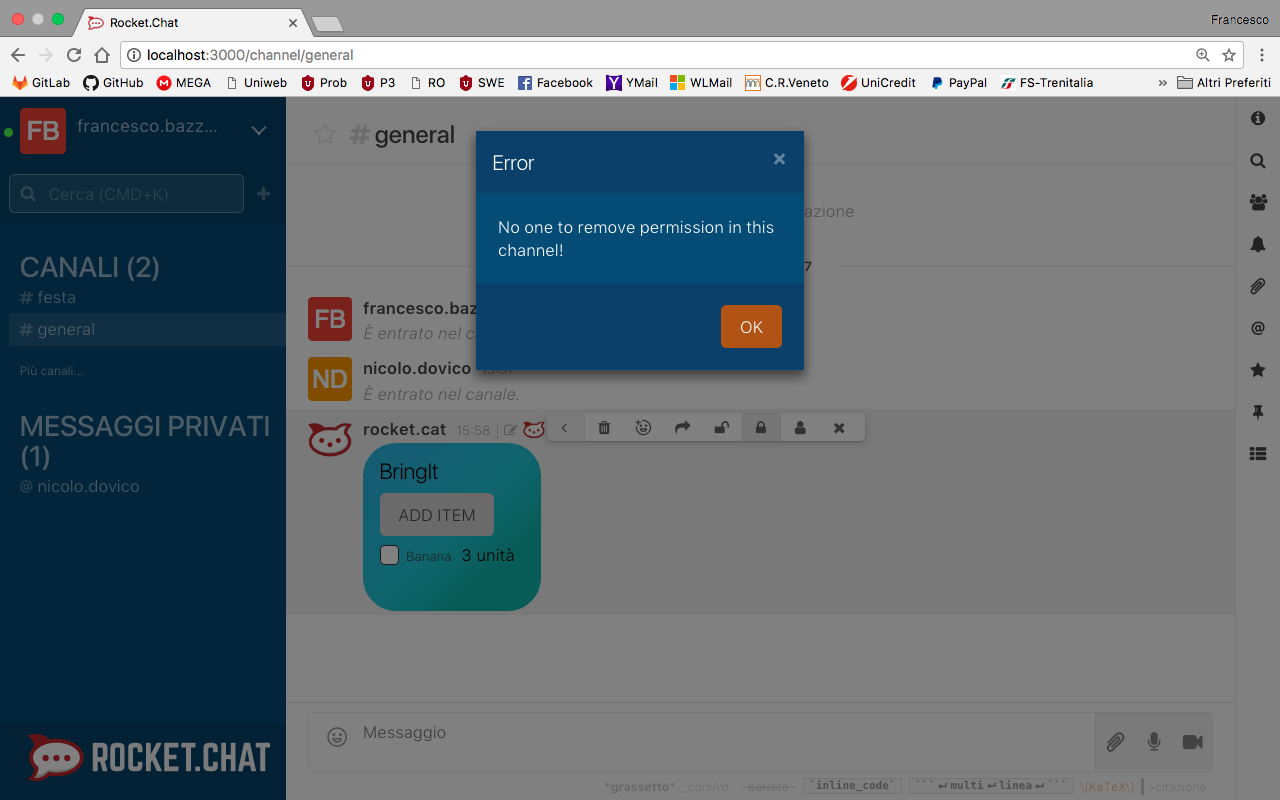
\includegraphics[width=\textwidth]{Sections/3-HowToUse/Images/permission_remove_error.png}
  \caption{Error shown if there are no people you can remove the permissions from.}
\end{figure}


\end{document}
